\documentclass[twoside]{book}

% Packages required by doxygen
\usepackage{fixltx2e}
\usepackage{calc}
\usepackage{doxygen}
\usepackage[export]{adjustbox} % also loads graphicx
\usepackage{graphicx}
\usepackage[utf8]{inputenc}
\usepackage{makeidx}
\usepackage{multicol}
\usepackage{multirow}
\PassOptionsToPackage{warn}{textcomp}
\usepackage{textcomp}
\usepackage[nointegrals]{wasysym}
\usepackage[table]{xcolor}

% Font selection
\usepackage[T1]{fontenc}
\usepackage[scaled=.90]{helvet}
\usepackage{courier}
\usepackage{amssymb}
\usepackage{sectsty}
\renewcommand{\familydefault}{\sfdefault}
\allsectionsfont{%
  \fontseries{bc}\selectfont%
  \color{darkgray}%
}
\renewcommand{\DoxyLabelFont}{%
  \fontseries{bc}\selectfont%
  \color{darkgray}%
}
\newcommand{\+}{\discretionary{\mbox{\scriptsize$\hookleftarrow$}}{}{}}

% Page & text layout
\usepackage{geometry}
\geometry{%
  a4paper,%
  top=2.5cm,%
  bottom=2.5cm,%
  left=2.5cm,%
  right=2.5cm%
}
\tolerance=750
\hfuzz=15pt
\hbadness=750
\setlength{\emergencystretch}{15pt}
\setlength{\parindent}{0cm}
\setlength{\parskip}{3ex plus 2ex minus 2ex}
\makeatletter
\renewcommand{\paragraph}{%
  \@startsection{paragraph}{4}{0ex}{-1.0ex}{1.0ex}{%
    \normalfont\normalsize\bfseries\SS@parafont%
  }%
}
\renewcommand{\subparagraph}{%
  \@startsection{subparagraph}{5}{0ex}{-1.0ex}{1.0ex}{%
    \normalfont\normalsize\bfseries\SS@subparafont%
  }%
}
\makeatother

% Headers & footers
\usepackage{fancyhdr}
\pagestyle{fancyplain}
\fancyhead[LE]{\fancyplain{}{\bfseries\thepage}}
\fancyhead[CE]{\fancyplain{}{}}
\fancyhead[RE]{\fancyplain{}{\bfseries\leftmark}}
\fancyhead[LO]{\fancyplain{}{\bfseries\rightmark}}
\fancyhead[CO]{\fancyplain{}{}}
\fancyhead[RO]{\fancyplain{}{\bfseries\thepage}}
\fancyfoot[LE]{\fancyplain{}{}}
\fancyfoot[CE]{\fancyplain{}{}}
\fancyfoot[RE]{\fancyplain{}{\bfseries\scriptsize Generated by Doxygen }}
\fancyfoot[LO]{\fancyplain{}{\bfseries\scriptsize Generated by Doxygen }}
\fancyfoot[CO]{\fancyplain{}{}}
\fancyfoot[RO]{\fancyplain{}{}}
\renewcommand{\footrulewidth}{0.4pt}
\renewcommand{\chaptermark}[1]{%
  \markboth{#1}{}%
}
\renewcommand{\sectionmark}[1]{%
  \markright{\thesection\ #1}%
}

% Indices & bibliography
\usepackage{natbib}
\usepackage[titles]{tocloft}
\setcounter{tocdepth}{3}
\setcounter{secnumdepth}{5}
\makeindex

% Hyperlinks (required, but should be loaded last)
\usepackage{ifpdf}
\ifpdf
  \usepackage[pdftex,pagebackref=true]{hyperref}
\else
  \usepackage[ps2pdf,pagebackref=true]{hyperref}
\fi
\hypersetup{%
  colorlinks=true,%
  linkcolor=blue,%
  citecolor=blue,%
  unicode%
}

% Custom commands
\newcommand{\clearemptydoublepage}{%
  \newpage{\pagestyle{empty}\cleardoublepage}%
}

\usepackage{caption}
\captionsetup{labelsep=space,justification=centering,font={bf},singlelinecheck=off,skip=4pt,position=top}

%===== C O N T E N T S =====

\begin{document}

% Titlepage & ToC
\hypersetup{pageanchor=false,
             bookmarksnumbered=true,
             pdfencoding=unicode
            }
\pagenumbering{alph}
\begin{titlepage}
\vspace*{7cm}
\begin{center}%
{\Large Little\+Tank \\[1ex]\large 0.\+1 }\\
\vspace*{1cm}
{\large Generated by Doxygen 1.8.13}\\
\end{center}
\end{titlepage}
\clearemptydoublepage
\pagenumbering{roman}
\tableofcontents
\clearemptydoublepage
\pagenumbering{arabic}
\hypersetup{pageanchor=true}

%--- Begin generated contents ---
\chapter{Namespace Index}
\section{Namespace List}
Here is a list of all documented namespaces with brief descriptions\+:\begin{DoxyCompactList}
\item\contentsline{section}{\hyperlink{namespacestate}{state} \\*Espace de nommage regroupant les données représentant l\textquotesingle{}état du jeu }{\pageref{namespacestate}}{}
\end{DoxyCompactList}

\chapter{Hierarchical Index}
\section{Class Hierarchy}
This inheritance list is sorted roughly, but not completely, alphabetically\+:\begin{DoxyCompactList}
\item \contentsline{section}{state\+:\+:Element}{\pageref{classstate_1_1_element}}{}
\begin{DoxyCompactList}
\item \contentsline{section}{Destructible}{\pageref{class_destructible}}{}
\begin{DoxyCompactList}
\item \contentsline{section}{Projectile}{\pageref{class_projectile}}{}
\end{DoxyCompactList}
\item \contentsline{section}{state\+:\+:Static\+Element}{\pageref{classstate_1_1_static_element}}{}
\begin{DoxyCompactList}
\item \contentsline{section}{state\+:\+:Obstacle}{\pageref{classstate_1_1_obstacle}}{}
\item \contentsline{section}{state\+:\+:Space}{\pageref{classstate_1_1_space}}{}
\end{DoxyCompactList}
\item \contentsline{section}{state\+:\+:Tank}{\pageref{classstate_1_1_tank}}{}
\end{DoxyCompactList}
\item \contentsline{section}{state\+:\+:Observable}{\pageref{classstate_1_1_observable}}{}
\begin{DoxyCompactList}
\item \contentsline{section}{state\+:\+:Element\+List}{\pageref{classstate_1_1_element_list}}{}
\item \contentsline{section}{state\+:\+:Global\+State}{\pageref{classstate_1_1_global_state}}{}
\item \contentsline{section}{state\+:\+:List\+Element}{\pageref{classstate_1_1_list_element}}{}
\begin{DoxyCompactList}
\item \contentsline{section}{state\+:\+:Element\+Grid}{\pageref{classstate_1_1_element_grid}}{}
\item \contentsline{section}{state\+:\+:Element\+Named\+List}{\pageref{classstate_1_1_element_named_list}}{}
\end{DoxyCompactList}
\end{DoxyCompactList}
\item \contentsline{section}{state\+:\+:State\+Event}{\pageref{classstate_1_1_state_event}}{}
\begin{DoxyCompactList}
\item \contentsline{section}{state\+:\+:Element\+Event}{\pageref{classstate_1_1_element_event}}{}
\item \contentsline{section}{state\+:\+:Projectile\+Event}{\pageref{classstate_1_1_projectile_event}}{}
\end{DoxyCompactList}
\item \contentsline{section}{state\+:\+:State\+Observer}{\pageref{classstate_1_1_state_observer}}{}
\end{DoxyCompactList}

\chapter{Class Index}
\section{Class List}
Here are the classes, structs, unions and interfaces with brief descriptions\+:\begin{DoxyCompactList}
\item\contentsline{section}{\hyperlink{class_destructible}{Destructible} }{\pageref{class_destructible}}{}
\item\contentsline{section}{\hyperlink{classstate_1_1_element}{state\+::\+Element} \\*Class \hyperlink{classstate_1_1_element}{Element} -\/ }{\pageref{classstate_1_1_element}}{}
\item\contentsline{section}{\hyperlink{classstate_1_1_element_event}{state\+::\+Element\+Event} \\*Class \hyperlink{classstate_1_1_element_event}{Element\+Event} -\/ Event \char`\"{}\+Element\+\_\+\+Changed\char`\"{} }{\pageref{classstate_1_1_element_event}}{}
\item\contentsline{section}{\hyperlink{classstate_1_1_element_grid}{state\+::\+Element\+Grid} \\*Class \hyperlink{classstate_1_1_element_grid}{Element\+Grid} -\/ List of Elements with a height and witdh }{\pageref{classstate_1_1_element_grid}}{}
\item\contentsline{section}{\hyperlink{classstate_1_1_element_list}{state\+::\+Element\+List} \\*Class \hyperlink{classstate_1_1_element_list}{Element\+List} -\/ List of Elements }{\pageref{classstate_1_1_element_list}}{}
\item\contentsline{section}{\hyperlink{classstate_1_1_element_named_list}{state\+::\+Element\+Named\+List} }{\pageref{classstate_1_1_element_named_list}}{}
\item\contentsline{section}{\hyperlink{classstate_1_1_global_state}{state\+::\+Global\+State} \\*Class State -\/ Store the list of the elements of the background (grid) and the list of the tank(mobiles) }{\pageref{classstate_1_1_global_state}}{}
\item\contentsline{section}{\hyperlink{classstate_1_1_list_element}{state\+::\+List\+Element} \\*Class \hyperlink{classstate_1_1_element_list}{Element\+List} -\/ List of Elements }{\pageref{classstate_1_1_list_element}}{}
\item\contentsline{section}{\hyperlink{classstate_1_1_observable}{state\+::\+Observable} \\*Class \hyperlink{classstate_1_1_observable}{Observable} -\/ List of the class\textquotesingle{}s observers }{\pageref{classstate_1_1_observable}}{}
\item\contentsline{section}{\hyperlink{classstate_1_1_obstacle}{state\+::\+Obstacle} \\*Class \hyperlink{classstate_1_1_obstacle}{Obstacle} -\/ }{\pageref{classstate_1_1_obstacle}}{}
\item\contentsline{section}{\hyperlink{class_projectile}{Projectile} }{\pageref{class_projectile}}{}
\item\contentsline{section}{\hyperlink{classstate_1_1_projectile_event}{state\+::\+Projectile\+Event} \\*Class \hyperlink{classstate_1_1_projectile_event}{Projectile\+Event} -\/ Event \char`\"{}\+Projectile\+\_\+\+Event\char`\"{} }{\pageref{classstate_1_1_projectile_event}}{}
\item\contentsline{section}{\hyperlink{classstate_1_1_space}{state\+::\+Space} \\*Classe representant les elements traversable }{\pageref{classstate_1_1_space}}{}
\item\contentsline{section}{\hyperlink{classstate_1_1_state_event}{state\+::\+State\+Event} \\*Class \hyperlink{classstate_1_1_state_event}{State\+Event} -\/ Event concerning the state }{\pageref{classstate_1_1_state_event}}{}
\item\contentsline{section}{\hyperlink{classstate_1_1_state_observer}{state\+::\+State\+Observer} \\*Class \hyperlink{classstate_1_1_state_observer}{State\+Observer} -\/ }{\pageref{classstate_1_1_state_observer}}{}
\item\contentsline{section}{\hyperlink{classstate_1_1_static_element}{state\+::\+Static\+Element} \\*Class \hyperlink{classstate_1_1_static_element}{Static\+Element} -\/ }{\pageref{classstate_1_1_static_element}}{}
\item\contentsline{section}{\hyperlink{classstate_1_1_tank}{state\+::\+Tank} \\*Class \hyperlink{classstate_1_1_tank}{Tank} -\/ }{\pageref{classstate_1_1_tank}}{}
\end{DoxyCompactList}

\chapter{File Index}
\section{File List}
Here is a list of all documented files with brief descriptions\+:\begin{DoxyCompactList}
\item\contentsline{section}{C\+:/\+Users/corentin/\+Desktop/projet tank/src modif/\+Tank\+State/{\bfseries state.\+h} }{\pageref{state_8h}}{}
\item\contentsline{section}{C\+:/\+Users/corentin/\+Desktop/projet tank/src modif/\+Tank\+State/include/{\bfseries Destructible.\+h} }{\pageref{_destructible_8h}}{}
\item\contentsline{section}{C\+:/\+Users/corentin/\+Desktop/projet tank/src modif/\+Tank\+State/include/{\bfseries Element.\+h} }{\pageref{_element_8h}}{}
\item\contentsline{section}{C\+:/\+Users/corentin/\+Desktop/projet tank/src modif/\+Tank\+State/include/{\bfseries Element\+Event.\+h} }{\pageref{_element_event_8h}}{}
\item\contentsline{section}{C\+:/\+Users/corentin/\+Desktop/projet tank/src modif/\+Tank\+State/include/{\bfseries Element\+Grid.\+h} }{\pageref{_element_grid_8h}}{}
\item\contentsline{section}{C\+:/\+Users/corentin/\+Desktop/projet tank/src modif/\+Tank\+State/include/{\bfseries Element\+List.\+h} }{\pageref{_element_list_8h}}{}
\item\contentsline{section}{C\+:/\+Users/corentin/\+Desktop/projet tank/src modif/\+Tank\+State/include/{\bfseries Element\+Named\+List.\+h} }{\pageref{_element_named_list_8h}}{}
\item\contentsline{section}{C\+:/\+Users/corentin/\+Desktop/projet tank/src modif/\+Tank\+State/include/{\bfseries Global\+State.\+h} }{\pageref{_global_state_8h}}{}
\item\contentsline{section}{C\+:/\+Users/corentin/\+Desktop/projet tank/src modif/\+Tank\+State/include/{\bfseries List\+Element.\+h} }{\pageref{_list_element_8h}}{}
\item\contentsline{section}{C\+:/\+Users/corentin/\+Desktop/projet tank/src modif/\+Tank\+State/include/{\bfseries List\+Type.\+h} }{\pageref{_list_type_8h}}{}
\item\contentsline{section}{C\+:/\+Users/corentin/\+Desktop/projet tank/src modif/\+Tank\+State/include/{\bfseries Observable.\+h} }{\pageref{_observable_8h}}{}
\item\contentsline{section}{C\+:/\+Users/corentin/\+Desktop/projet tank/src modif/\+Tank\+State/include/{\bfseries Obstacle.\+h} }{\pageref{_obstacle_8h}}{}
\item\contentsline{section}{C\+:/\+Users/corentin/\+Desktop/projet tank/src modif/\+Tank\+State/include/{\bfseries Obstacle\+Type\+Id.\+h} }{\pageref{_obstacle_type_id_8h}}{}
\item\contentsline{section}{C\+:/\+Users/corentin/\+Desktop/projet tank/src modif/\+Tank\+State/include/{\bfseries Orientation.\+h} }{\pageref{_orientation_8h}}{}
\item\contentsline{section}{C\+:/\+Users/corentin/\+Desktop/projet tank/src modif/\+Tank\+State/include/{\bfseries Projectile.\+h} }{\pageref{_projectile_8h}}{}
\item\contentsline{section}{C\+:/\+Users/corentin/\+Desktop/projet tank/src modif/\+Tank\+State/include/{\bfseries Projectile\+Event.\+h} }{\pageref{_projectile_event_8h}}{}
\item\contentsline{section}{C\+:/\+Users/corentin/\+Desktop/projet tank/src modif/\+Tank\+State/include/{\bfseries Space.\+h} }{\pageref{_space_8h}}{}
\item\contentsline{section}{C\+:/\+Users/corentin/\+Desktop/projet tank/src modif/\+Tank\+State/include/{\bfseries Space\+Type\+Id.\+h} }{\pageref{_space_type_id_8h}}{}
\item\contentsline{section}{C\+:/\+Users/corentin/\+Desktop/projet tank/src modif/\+Tank\+State/include/{\bfseries State\+Event.\+h} }{\pageref{_state_event_8h}}{}
\item\contentsline{section}{C\+:/\+Users/corentin/\+Desktop/projet tank/src modif/\+Tank\+State/include/{\bfseries State\+Event\+Id.\+h} }{\pageref{_state_event_id_8h}}{}
\item\contentsline{section}{C\+:/\+Users/corentin/\+Desktop/projet tank/src modif/\+Tank\+State/include/{\bfseries State\+Observer.\+h} }{\pageref{_state_observer_8h}}{}
\item\contentsline{section}{C\+:/\+Users/corentin/\+Desktop/projet tank/src modif/\+Tank\+State/include/{\bfseries Static\+Element.\+h} }{\pageref{_static_element_8h}}{}
\item\contentsline{section}{C\+:/\+Users/corentin/\+Desktop/projet tank/src modif/\+Tank\+State/include/{\bfseries Tank.\+h} }{\pageref{_tank_8h}}{}
\item\contentsline{section}{C\+:/\+Users/corentin/\+Desktop/projet tank/src modif/\+Tank\+State/include/{\bfseries Tank\+Type\+Id.\+h} }{\pageref{_tank_type_id_8h}}{}
\item\contentsline{section}{C\+:/\+Users/corentin/\+Desktop/projet tank/src modif/\+Tank\+State/include/{\bfseries Type\+Id.\+h} }{\pageref{_type_id_8h}}{}
\item\contentsline{section}{C\+:/\+Users/corentin/\+Desktop/projet tank/src modif/\+Tank\+State/src/\hyperlink{_space_8cpp}{Space.\+cpp} \\*Element Space }{\pageref{_space_8cpp}}{}
\end{DoxyCompactList}

\chapter{Namespace Documentation}
\hypertarget{namespacestate}{}\section{state Namespace Reference}
\label{namespacestate}\index{state@{state}}


Espace de nommage regroupant les données représentant l\textquotesingle{}état du jeu.  


\subsection*{Classes}
\begin{DoxyCompactItemize}
\item 
class \hyperlink{classstate_1_1_element}{Element}
\begin{DoxyCompactList}\small\item\em class \hyperlink{classstate_1_1_element}{Element} -\/ \end{DoxyCompactList}\item 
class \hyperlink{classstate_1_1_element_event}{Element\+Event}
\begin{DoxyCompactList}\small\item\em class \hyperlink{classstate_1_1_element_event}{Element\+Event} -\/ Event \char`\"{}\+Element\+\_\+\+Changed\char`\"{} \end{DoxyCompactList}\item 
class \hyperlink{classstate_1_1_element_grid}{Element\+Grid}
\begin{DoxyCompactList}\small\item\em class \hyperlink{classstate_1_1_element_grid}{Element\+Grid} -\/ List of Elements with a height and witdh \end{DoxyCompactList}\item 
class \hyperlink{classstate_1_1_element_list}{Element\+List}
\begin{DoxyCompactList}\small\item\em class \hyperlink{classstate_1_1_element_list}{Element\+List} -\/ List of Elements \end{DoxyCompactList}\item 
class \hyperlink{classstate_1_1_element_named_list}{Element\+Named\+List}
\item 
class \hyperlink{classstate_1_1_global_state}{Global\+State}
\begin{DoxyCompactList}\small\item\em class State -\/ Store the list of the elements of the background (grid) and the list of the tank(mobiles) \end{DoxyCompactList}\item 
class \hyperlink{classstate_1_1_list_element}{List\+Element}
\begin{DoxyCompactList}\small\item\em class \hyperlink{classstate_1_1_element_list}{Element\+List} -\/ List of Elements \end{DoxyCompactList}\item 
class \hyperlink{classstate_1_1_observable}{Observable}
\begin{DoxyCompactList}\small\item\em class \hyperlink{classstate_1_1_observable}{Observable} -\/ List of the class\textquotesingle{}s observers \end{DoxyCompactList}\item 
class \hyperlink{classstate_1_1_obstacle}{Obstacle}
\begin{DoxyCompactList}\small\item\em class \hyperlink{classstate_1_1_obstacle}{Obstacle} -\/ \end{DoxyCompactList}\item 
class \hyperlink{classstate_1_1_projectile_event}{Projectile\+Event}
\begin{DoxyCompactList}\small\item\em class \hyperlink{classstate_1_1_projectile_event}{Projectile\+Event} -\/ Event \char`\"{}\+Projectile\+\_\+\+Event\char`\"{} \end{DoxyCompactList}\item 
class \hyperlink{classstate_1_1_space}{Space}
\begin{DoxyCompactList}\small\item\em classe representant les elements traversable \end{DoxyCompactList}\item 
class \hyperlink{classstate_1_1_state_event}{State\+Event}
\begin{DoxyCompactList}\small\item\em class \hyperlink{classstate_1_1_state_event}{State\+Event} -\/ Event concerning the state \end{DoxyCompactList}\item 
class \hyperlink{classstate_1_1_state_observer}{State\+Observer}
\begin{DoxyCompactList}\small\item\em class \hyperlink{classstate_1_1_state_observer}{State\+Observer} -\/ \end{DoxyCompactList}\item 
class \hyperlink{classstate_1_1_static_element}{Static\+Element}
\begin{DoxyCompactList}\small\item\em class \hyperlink{classstate_1_1_static_element}{Static\+Element} -\/ \end{DoxyCompactList}\item 
class \hyperlink{classstate_1_1_tank}{Tank}
\begin{DoxyCompactList}\small\item\em class \hyperlink{classstate_1_1_tank}{Tank} -\/ \end{DoxyCompactList}\end{DoxyCompactItemize}
\subsection*{Enumerations}
\begin{DoxyCompactItemize}
\item 
\mbox{\Hypertarget{namespacestate_acdd67f28d032af61c857718a6945df94}\label{namespacestate_acdd67f28d032af61c857718a6945df94}} 
enum {\bfseries List\+Type} \{ {\bfseries terrestre} = 0, 
{\bfseries aerien} = 1, 
{\bfseries projectile} = 2, 
{\bfseries paysage} = 3
 \}
\item 
\mbox{\Hypertarget{namespacestate_a83db3ada133da88934c6ab78f39488af}\label{namespacestate_a83db3ada133da88934c6ab78f39488af}} 
enum {\bfseries Obstacle\+Type\+Id} \{ {\bfseries sand} = 1, 
{\bfseries border} = 2
 \}
\item 
\mbox{\Hypertarget{namespacestate_a356fdb25c53a0d3f532a2f9770fdd63d}\label{namespacestate_a356fdb25c53a0d3f532a2f9770fdd63d}} 
enum {\bfseries Orientation} \{ {\bfseries left\+\_\+down} =1, 
{\bfseries left\+\_\+up} = 2, 
{\bfseries right\+\_\+down} = 3, 
{\bfseries right\+\_\+up} = 4
 \}
\item 
\mbox{\Hypertarget{namespacestate_a1648cef1bd53299cc6dfd90eeee3c0f1}\label{namespacestate_a1648cef1bd53299cc6dfd90eeee3c0f1}} 
enum {\bfseries Space\+Type\+Id} \{ {\bfseries sky} = 1, 
{\bfseries greenery} = 2
 \}
\item 
\mbox{\Hypertarget{namespacestate_a5a660a8300e8f8d4be0e2ec73800de09}\label{namespacestate_a5a660a8300e8f8d4be0e2ec73800de09}} 
enum {\bfseries State\+Event\+Id} \{ {\bfseries Level\+\_\+\+Changed} = 1, 
{\bfseries Element\+\_\+\+Changed} = 2, 
{\bfseries Pv\+\_\+\+Changed} = 3, 
{\bfseries Projectile\+\_\+\+Event} = 4
 \}
\item 
\mbox{\Hypertarget{namespacestate_aff734372f7f087a0e1f635cb9716dd1a}\label{namespacestate_aff734372f7f087a0e1f635cb9716dd1a}} 
enum {\bfseries Tank\+Type\+Id} \{ {\bfseries Little\+\_\+tank\+\_\+green} = 1, 
{\bfseries Little\+\_\+tank\+\_\+grey} = 2, 
{\bfseries Big\+\_\+tank\+\_\+green} = 3, 
{\bfseries Big\+\_\+tank\+\_\+grey} = 4
 \}
\item 
\mbox{\Hypertarget{namespacestate_a52ac81a498c9b1ebe1b905a40439c7d3}\label{namespacestate_a52ac81a498c9b1ebe1b905a40439c7d3}} 
enum {\bfseries Type\+Id} \{ {\bfseries obstacle} = 1, 
{\bfseries space} = 2, 
{\bfseries tank} = 3
 \}
\end{DoxyCompactItemize}


\subsection{Detailed Description}
Espace de nommage regroupant les données représentant l\textquotesingle{}état du jeu. 
\chapter{Class Documentation}
\hypertarget{class_destructible}{}\section{Destructible Class Reference}
\label{class_destructible}\index{Destructible@{Destructible}}
Inheritance diagram for Destructible\+:\begin{figure}[H]
\begin{center}
\leavevmode
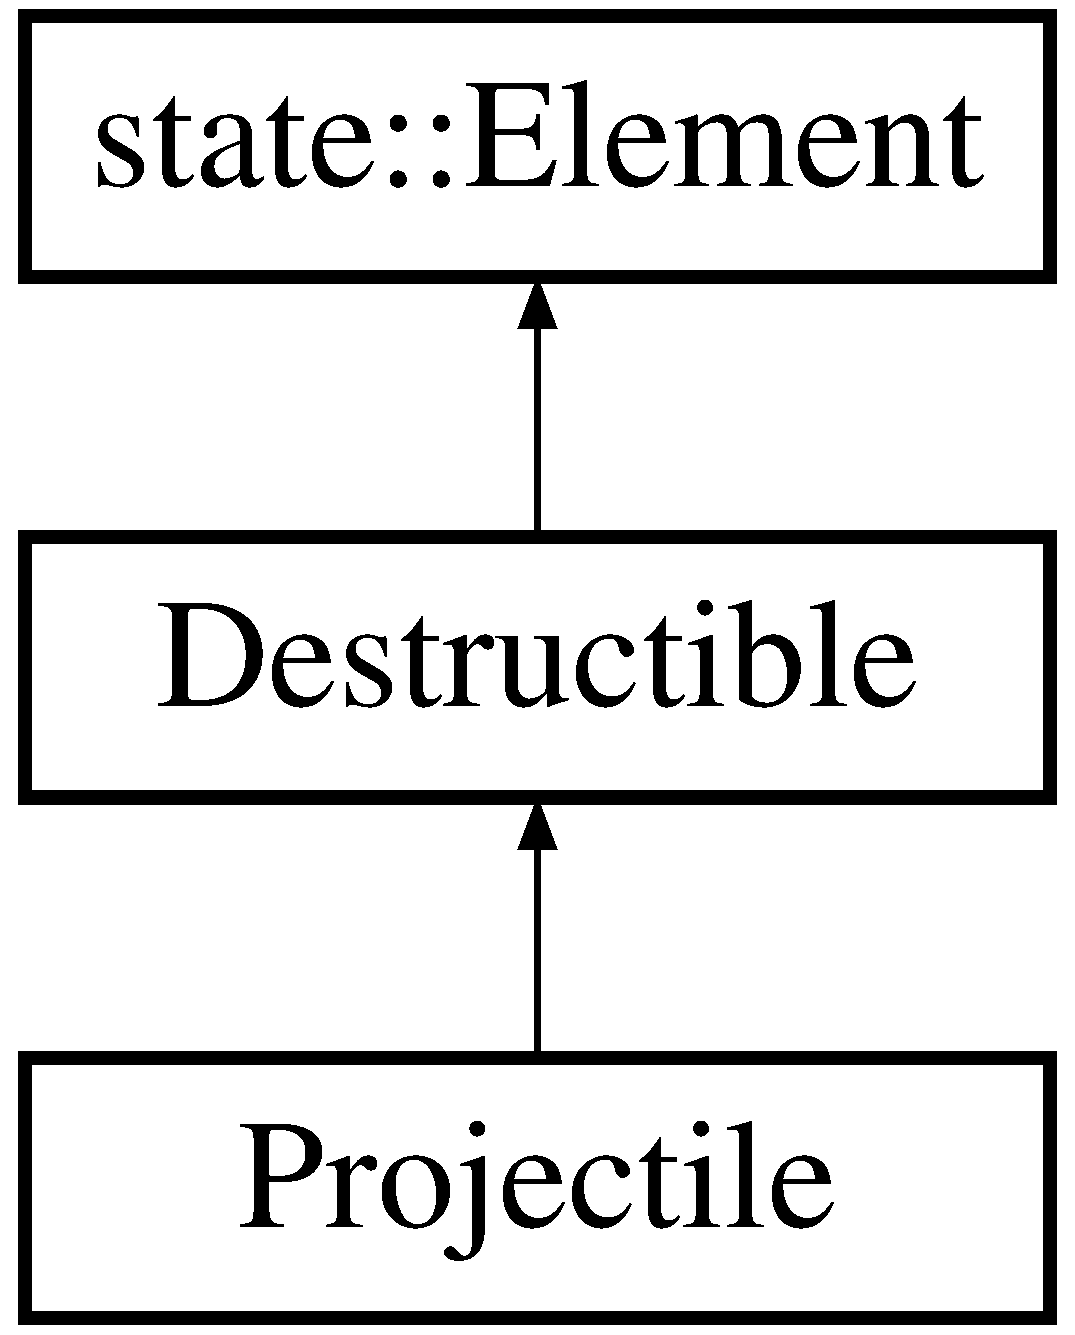
\includegraphics[height=3.000000cm]{class_destructible}
\end{center}
\end{figure}
\subsection*{Public Member Functions}
\begin{DoxyCompactItemize}
\item 
\mbox{\Hypertarget{class_destructible_a88c03b7b5cbf35373979b8bbabff43e7}\label{class_destructible_a88c03b7b5cbf35373979b8bbabff43e7}} 
{\bfseries Destructible} (int x, int y, int pv, int effect)
\item 
\mbox{\Hypertarget{class_destructible_a589a43ef2fc0bd441ffc456aa3f8183a}\label{class_destructible_a589a43ef2fc0bd441ffc456aa3f8183a}} 
int \hyperlink{class_destructible_a589a43ef2fc0bd441ffc456aa3f8183a}{Getpv} ()
\begin{DoxyCompactList}\small\item\em Getteur. \end{DoxyCompactList}\item 
\mbox{\Hypertarget{class_destructible_a3422fe6ceac29d16c5d1bcb2457c2f8f}\label{class_destructible_a3422fe6ceac29d16c5d1bcb2457c2f8f}} 
void {\bfseries Setpv} (int val)
\item 
\mbox{\Hypertarget{class_destructible_a6dc11130f41a51da85cc40010d3ca3b4}\label{class_destructible_a6dc11130f41a51da85cc40010d3ca3b4}} 
int {\bfseries Geteffect} ()
\item 
\mbox{\Hypertarget{class_destructible_a828ea57137534a4639ab736dbb394733}\label{class_destructible_a828ea57137534a4639ab736dbb394733}} 
void {\bfseries Seteffect} (int val)
\end{DoxyCompactItemize}
\subsection*{Additional Inherited Members}


The documentation for this class was generated from the following files\+:\begin{DoxyCompactItemize}
\item 
C\+:/\+Users/corentin/\+Desktop/projet tank/src modif/\+Tank\+State/include/Destructible.\+h\item 
C\+:/\+Users/corentin/\+Desktop/projet tank/src modif/\+Tank\+State/src/Destructible.\+cpp\end{DoxyCompactItemize}

\hypertarget{classstate_1_1_element}{}\section{state\+:\+:Element Class Reference}
\label{classstate_1_1_element}\index{state\+::\+Element@{state\+::\+Element}}


class \hyperlink{classstate_1_1_element}{Element} -\/  




{\ttfamily \#include $<$Element.\+h$>$}

Inheritance diagram for state\+:\+:Element\+:\begin{figure}[H]
\begin{center}
\leavevmode
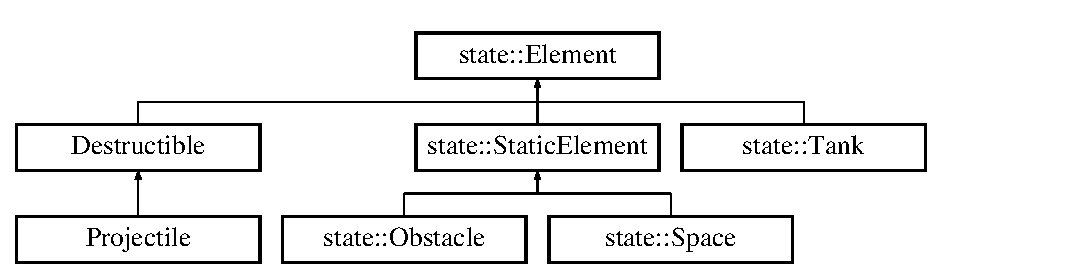
\includegraphics[height=3.000000cm]{classstate_1_1_element}
\end{center}
\end{figure}
\subsection*{Public Member Functions}
\begin{DoxyCompactItemize}
\item 
\mbox{\Hypertarget{classstate_1_1_element_a21519707215e66543dbd8f3c7a90a101}\label{classstate_1_1_element_a21519707215e66543dbd8f3c7a90a101}} 
virtual Type\+Id {\bfseries get\+Type\+Id} () const =0
\item 
\mbox{\Hypertarget{classstate_1_1_element_a8f24736ef9d139c43de6170bbf12b934}\label{classstate_1_1_element_a8f24736ef9d139c43de6170bbf12b934}} 
virtual bool {\bfseries is\+Static} () const =0
\item 
\mbox{\Hypertarget{classstate_1_1_element_ae7bba399afdeb9e002c28a3d0d389fd0}\label{classstate_1_1_element_ae7bba399afdeb9e002c28a3d0d389fd0}} 
bool \hyperlink{classstate_1_1_element_ae7bba399afdeb9e002c28a3d0d389fd0}{is\+Composite} ()
\begin{DoxyCompactList}\small\item\em Permet de vérifié si cela est composite. \end{DoxyCompactList}\item 
\mbox{\Hypertarget{classstate_1_1_element_ad255661bd2e71f48014e6a80dd914ab0}\label{classstate_1_1_element_ad255661bd2e71f48014e6a80dd914ab0}} 
int {\bfseries getX} () const
\item 
\mbox{\Hypertarget{classstate_1_1_element_a064240b24695cc5c052fbfd4a55489f2}\label{classstate_1_1_element_a064240b24695cc5c052fbfd4a55489f2}} 
int {\bfseries getY} () const
\item 
\mbox{\Hypertarget{classstate_1_1_element_a96672cf4848c5566115c2ea3fec8161d}\label{classstate_1_1_element_a96672cf4848c5566115c2ea3fec8161d}} 
void {\bfseries setX} (int x)
\item 
\mbox{\Hypertarget{classstate_1_1_element_aa66f35989d8c833ef566c01e23e63e10}\label{classstate_1_1_element_aa66f35989d8c833ef566c01e23e63e10}} 
void {\bfseries setY} (int y)
\item 
\mbox{\Hypertarget{classstate_1_1_element_a0e2e8e4cc3e33c4ed57c49a876d09476}\label{classstate_1_1_element_a0e2e8e4cc3e33c4ed57c49a876d09476}} 
void \hyperlink{classstate_1_1_element_a0e2e8e4cc3e33c4ed57c49a876d09476}{moveX} (int dx)
\begin{DoxyCompactList}\small\item\em Permet de déplacer le bloc composite de dx. \end{DoxyCompactList}\item 
\mbox{\Hypertarget{classstate_1_1_element_a26f3b97d04d24f2d2ffa6513099778db}\label{classstate_1_1_element_a26f3b97d04d24f2d2ffa6513099778db}} 
void \hyperlink{classstate_1_1_element_a26f3b97d04d24f2d2ffa6513099778db}{moveY} (int dy)
\begin{DoxyCompactList}\small\item\em Permet de déplacer le bloc composite de dy. \end{DoxyCompactList}\item 
\mbox{\Hypertarget{classstate_1_1_element_a676d60d605e100796ba0962d7b383415}\label{classstate_1_1_element_a676d60d605e100796ba0962d7b383415}} 
bool \hyperlink{classstate_1_1_element_a676d60d605e100796ba0962d7b383415}{is\+Here} (int x, int y)
\begin{DoxyCompactList}\small\item\em Permet de vérifier la position pour un bloc composite. \end{DoxyCompactList}\item 
\mbox{\Hypertarget{classstate_1_1_element_ad4e348a88665a7b251d2a671ad910fae}\label{classstate_1_1_element_ad4e348a88665a7b251d2a671ad910fae}} 
std\+::vector$<$ \hyperlink{classstate_1_1_element}{Element} $\ast$ $>$ \hyperlink{classstate_1_1_element_ad4e348a88665a7b251d2a671ad910fae}{get\+Bloc} ()
\begin{DoxyCompactList}\small\item\em Renvoie le bloc entier. \end{DoxyCompactList}\item 
\mbox{\Hypertarget{classstate_1_1_element_a9d35c7951f1aeaeea9775f5151dee98b}\label{classstate_1_1_element_a9d35c7951f1aeaeea9775f5151dee98b}} 
bool \hyperlink{classstate_1_1_element_a9d35c7951f1aeaeea9775f5151dee98b}{add} (\hyperlink{classstate_1_1_element}{Element} $\ast$e)
\begin{DoxyCompactList}\small\item\em Ajoute un élément à la liste des membres (composite) \end{DoxyCompactList}\item 
\mbox{\Hypertarget{classstate_1_1_element_aa11351137acee5ddcf2f5b52fadfda3b}\label{classstate_1_1_element_aa11351137acee5ddcf2f5b52fadfda3b}} 
virtual \hyperlink{classstate_1_1_element}{Element} $\ast$ {\bfseries clone} () const =0
\end{DoxyCompactItemize}
\subsection*{Protected Attributes}
\begin{DoxyCompactItemize}
\item 
\mbox{\Hypertarget{classstate_1_1_element_aae18fab1d563f154f64760cf6b9d96c4}\label{classstate_1_1_element_aae18fab1d563f154f64760cf6b9d96c4}} 
int {\bfseries x}
\item 
\mbox{\Hypertarget{classstate_1_1_element_a726a92bb1fa8a574359760c16febd212}\label{classstate_1_1_element_a726a92bb1fa8a574359760c16febd212}} 
int {\bfseries y}
\item 
\mbox{\Hypertarget{classstate_1_1_element_a4fc0e453f7f839ef07e57ee9a95ee62c}\label{classstate_1_1_element_a4fc0e453f7f839ef07e57ee9a95ee62c}} 
std\+::vector$<$ \hyperlink{classstate_1_1_element}{Element} $\ast$ $>$ {\bfseries composite}
\end{DoxyCompactItemize}


\subsection{Detailed Description}
class \hyperlink{classstate_1_1_element}{Element} -\/ 

The documentation for this class was generated from the following files\+:\begin{DoxyCompactItemize}
\item 
C\+:/\+Users/corentin/\+Desktop/projet tank/src modif/\+Tank\+State/include/Element.\+h\item 
C\+:/\+Users/corentin/\+Desktop/projet tank/src modif/\+Tank\+State/src/Element.\+cpp\end{DoxyCompactItemize}

\hypertarget{classstate_1_1_element_event}{}\section{state\+:\+:Element\+Event Class Reference}
\label{classstate_1_1_element_event}\index{state\+::\+Element\+Event@{state\+::\+Element\+Event}}


class \hyperlink{classstate_1_1_element_event}{Element\+Event} -\/ Event \char`\"{}\+Element\+\_\+\+Changed\char`\"{}  




{\ttfamily \#include $<$Element\+Event.\+h$>$}

Inheritance diagram for state\+:\+:Element\+Event\+:\begin{figure}[H]
\begin{center}
\leavevmode
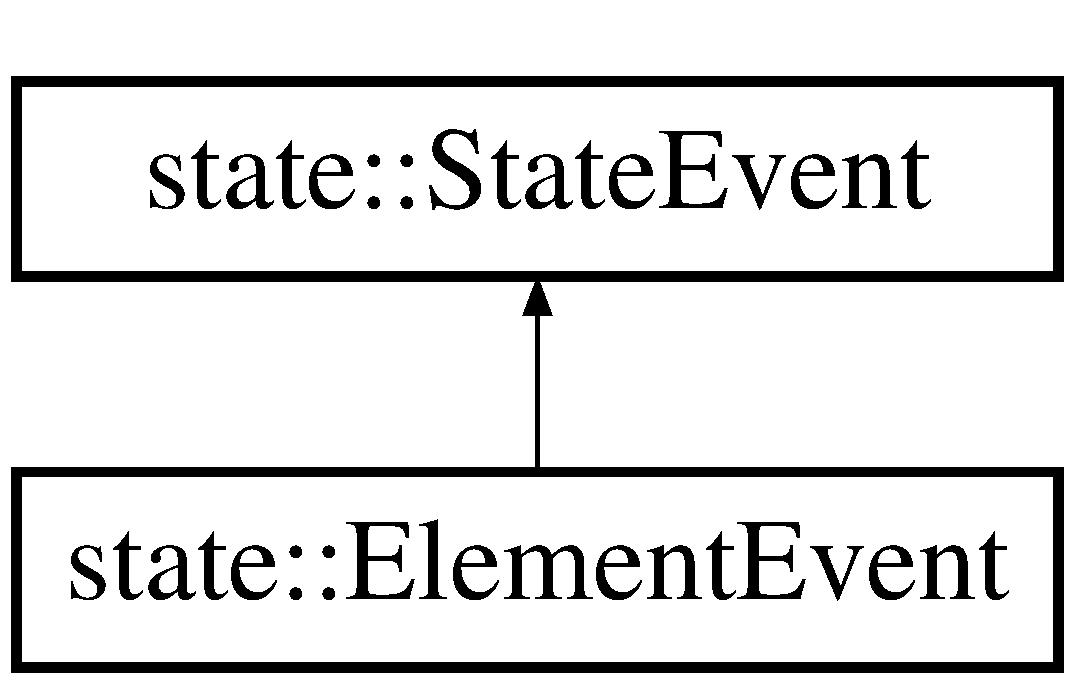
\includegraphics[height=2.000000cm]{classstate_1_1_element_event}
\end{center}
\end{figure}
\subsection*{Public Member Functions}
\begin{DoxyCompactItemize}
\item 
\mbox{\Hypertarget{classstate_1_1_element_event_a202d5ac87bb4d4622c980322b9171abb}\label{classstate_1_1_element_event_a202d5ac87bb4d4622c980322b9171abb}} 
{\bfseries Element\+Event} (const \hyperlink{classstate_1_1_list_element}{List\+Element} $\ast$list, int idx=-\/1)
\item 
\mbox{\Hypertarget{classstate_1_1_element_event_a41749106ecf73340ead82a6bd867d485}\label{classstate_1_1_element_event_a41749106ecf73340ead82a6bd867d485}} 
\hyperlink{classstate_1_1_state_event}{State\+Event} $\ast$ {\bfseries clone} () const
\end{DoxyCompactItemize}
\subsection*{Public Attributes}
\begin{DoxyCompactItemize}
\item 
\mbox{\Hypertarget{classstate_1_1_element_event_a616b97e30980909d9e0ff896672c50f1}\label{classstate_1_1_element_event_a616b97e30980909d9e0ff896672c50f1}} 
const \hyperlink{classstate_1_1_list_element}{List\+Element} $\ast$ {\bfseries list}
\item 
\mbox{\Hypertarget{classstate_1_1_element_event_a5df40bbf28979ba9e435a4f52a05878e}\label{classstate_1_1_element_event_a5df40bbf28979ba9e435a4f52a05878e}} 
int {\bfseries idx}
\end{DoxyCompactItemize}


\subsection{Detailed Description}
class \hyperlink{classstate_1_1_element_event}{Element\+Event} -\/ Event \char`\"{}\+Element\+\_\+\+Changed\char`\"{} 

The documentation for this class was generated from the following files\+:\begin{DoxyCompactItemize}
\item 
C\+:/\+Users/corentin/\+Desktop/projet tank/src modif/\+Tank\+State/include/Element\+Event.\+h\item 
C\+:/\+Users/corentin/\+Desktop/projet tank/src modif/\+Tank\+State/src/Element\+Event.\+cpp\end{DoxyCompactItemize}

\hypertarget{classstate_1_1_element_grid}{}\section{state\+:\+:Element\+Grid Class Reference}
\label{classstate_1_1_element_grid}\index{state\+::\+Element\+Grid@{state\+::\+Element\+Grid}}


class \hyperlink{classstate_1_1_element_grid}{Element\+Grid} -\/ List of Elements with a height and witdh  




{\ttfamily \#include $<$Element\+Grid.\+h$>$}

Inheritance diagram for state\+:\+:Element\+Grid\+:\begin{figure}[H]
\begin{center}
\leavevmode
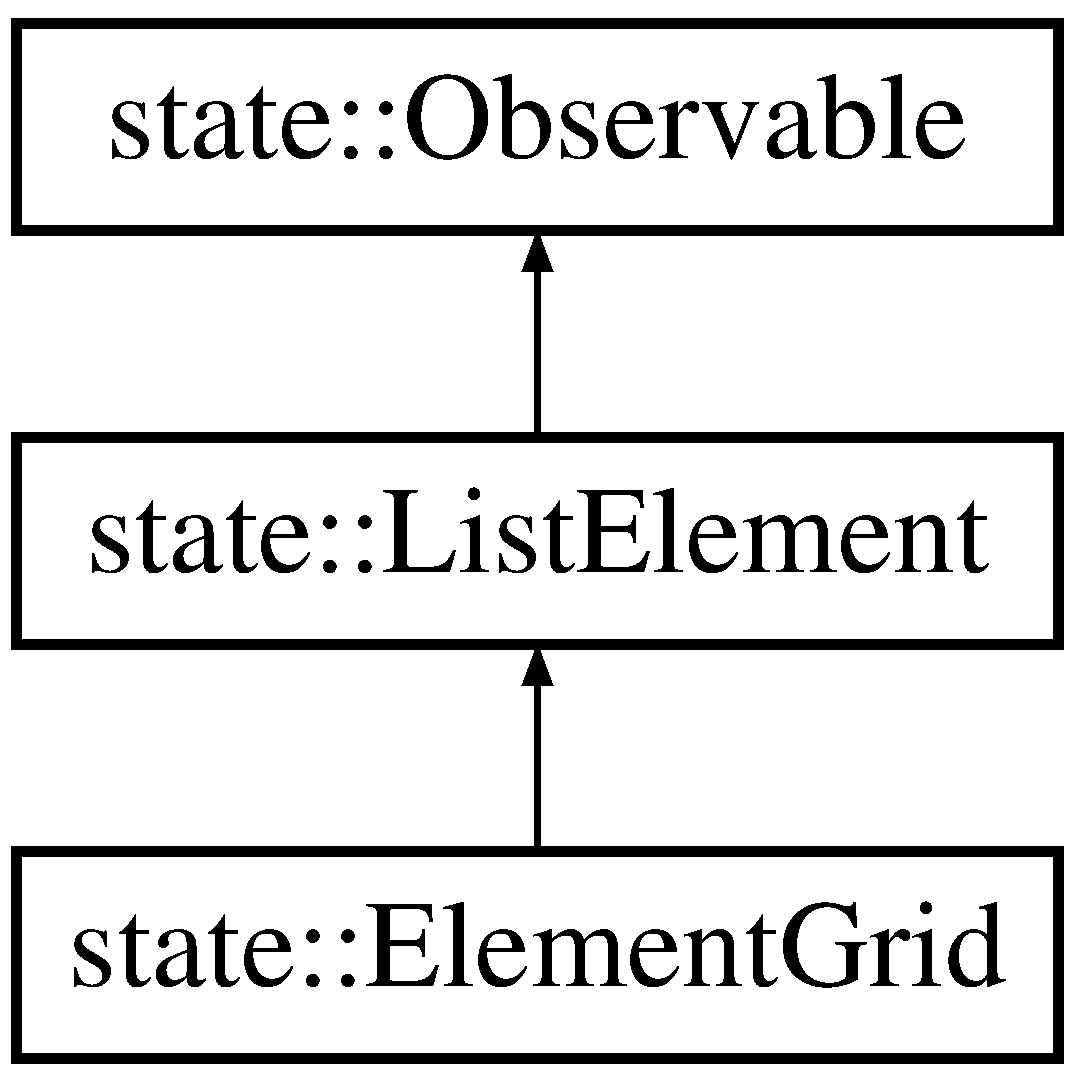
\includegraphics[height=3.000000cm]{classstate_1_1_element_grid}
\end{center}
\end{figure}
\subsection*{Public Member Functions}
\begin{DoxyCompactItemize}
\item 
\mbox{\Hypertarget{classstate_1_1_element_grid_a56dd28b11c12dcf5493fe263d6e00c93}\label{classstate_1_1_element_grid_a56dd28b11c12dcf5493fe263d6e00c93}} 
{\bfseries Element\+Grid} (\hyperlink{classstate_1_1_global_state}{Global\+State} \&s)
\item 
\mbox{\Hypertarget{classstate_1_1_element_grid_a223578d89ab0e706156e4a9ebd18192e}\label{classstate_1_1_element_grid_a223578d89ab0e706156e4a9ebd18192e}} 
int {\bfseries get\+Width} () const
\item 
\mbox{\Hypertarget{classstate_1_1_element_grid_a4eb505218a65d86686bbf75be79e5730}\label{classstate_1_1_element_grid_a4eb505218a65d86686bbf75be79e5730}} 
int {\bfseries get\+Height} () const
\item 
\mbox{\Hypertarget{classstate_1_1_element_grid_aea2a3f241f4852a8bef43a191b870bd2}\label{classstate_1_1_element_grid_aea2a3f241f4852a8bef43a191b870bd2}} 
\hyperlink{classstate_1_1_element}{Element} $\ast$ {\bfseries get\+Cell} (int i, int j) const
\item 
\mbox{\Hypertarget{classstate_1_1_element_grid_a276cbb60a6ebf0529520252bb62c35e6}\label{classstate_1_1_element_grid_a276cbb60a6ebf0529520252bb62c35e6}} 
bool {\bfseries is\+Space} (int i, int j) const
\item 
\mbox{\Hypertarget{classstate_1_1_element_grid_a60ed64fe49212644f7fb44f3aca40977}\label{classstate_1_1_element_grid_a60ed64fe49212644f7fb44f3aca40977}} 
void {\bfseries set\+Cell} (int i, int j, \hyperlink{classstate_1_1_element}{Element} $\ast$e)
\item 
\mbox{\Hypertarget{classstate_1_1_element_grid_a6c4fa8ef09a0b186ed0427bcaa9da694}\label{classstate_1_1_element_grid_a6c4fa8ef09a0b186ed0427bcaa9da694}} 
bool {\bfseries has\+Cell} (int i, int j) const
\item 
\mbox{\Hypertarget{classstate_1_1_element_grid_abd07f1879721724da8fb65f6100c27b7}\label{classstate_1_1_element_grid_abd07f1879721724da8fb65f6100c27b7}} 
void {\bfseries set\+Height} (int h)
\item 
\mbox{\Hypertarget{classstate_1_1_element_grid_a215baba29f16559346bd2562585f97c2}\label{classstate_1_1_element_grid_a215baba29f16559346bd2562585f97c2}} 
void {\bfseries set\+Width} (int w)
\item 
\mbox{\Hypertarget{classstate_1_1_element_grid_ab0bfc961842b2096404f2a12db81bb50}\label{classstate_1_1_element_grid_ab0bfc961842b2096404f2a12db81bb50}} 
void {\bfseries copy} (const \hyperlink{classstate_1_1_element_grid}{Element\+Grid} e)
\end{DoxyCompactItemize}
\subsection*{Protected Attributes}
\begin{DoxyCompactItemize}
\item 
\mbox{\Hypertarget{classstate_1_1_element_grid_acfd12b1d8a3af4bd4f554ed8ca593c51}\label{classstate_1_1_element_grid_acfd12b1d8a3af4bd4f554ed8ca593c51}} 
int {\bfseries width}
\item 
\mbox{\Hypertarget{classstate_1_1_element_grid_aad232b16857ba8243b2f0e7f833b4c0b}\label{classstate_1_1_element_grid_aad232b16857ba8243b2f0e7f833b4c0b}} 
int {\bfseries height}
\item 
\mbox{\Hypertarget{classstate_1_1_element_grid_a4d8735e4e069609c3898783317c467e7}\label{classstate_1_1_element_grid_a4d8735e4e069609c3898783317c467e7}} 
\hyperlink{classstate_1_1_global_state}{Global\+State} \& {\bfseries s}
\end{DoxyCompactItemize}


\subsection{Detailed Description}
class \hyperlink{classstate_1_1_element_grid}{Element\+Grid} -\/ List of Elements with a height and witdh 

The documentation for this class was generated from the following files\+:\begin{DoxyCompactItemize}
\item 
C\+:/\+Users/corentin/\+Desktop/projet tank/src modif/\+Tank\+State/include/Element\+Grid.\+h\item 
C\+:/\+Users/corentin/\+Desktop/projet tank/src modif/\+Tank\+State/src/Element\+Grid.\+cpp\end{DoxyCompactItemize}

\hypertarget{classstate_1_1_element_list}{}\section{state\+:\+:Element\+List Class Reference}
\label{classstate_1_1_element_list}\index{state\+::\+Element\+List@{state\+::\+Element\+List}}


class \hyperlink{classstate_1_1_element_list}{Element\+List} -\/ List of Elements  




{\ttfamily \#include $<$Element\+List.\+h$>$}

Inheritance diagram for state\+:\+:Element\+List\+:\begin{figure}[H]
\begin{center}
\leavevmode
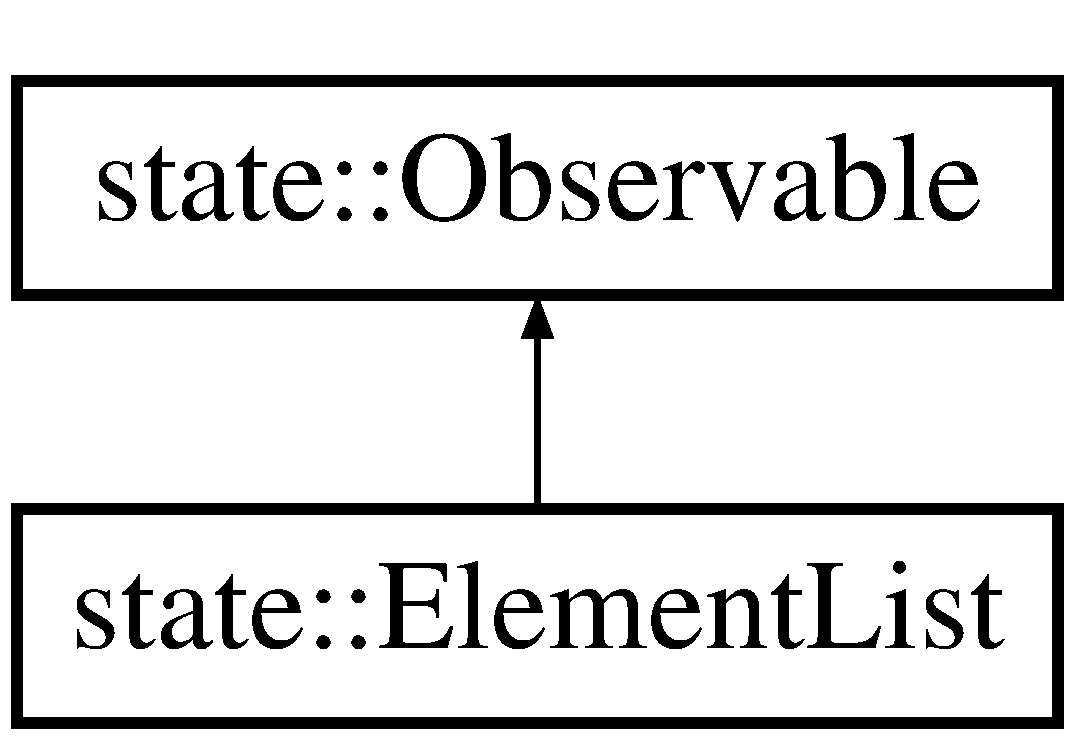
\includegraphics[height=2.000000cm]{classstate_1_1_element_list}
\end{center}
\end{figure}
\subsection*{Public Member Functions}
\begin{DoxyCompactItemize}
\item 
\mbox{\Hypertarget{classstate_1_1_element_list_abfb38469f7e90e8720147d043cfc99ec}\label{classstate_1_1_element_list_abfb38469f7e90e8720147d043cfc99ec}} 
{\bfseries Element\+List} (State \&s)
\item 
\mbox{\Hypertarget{classstate_1_1_element_list_a5e102ac6024b29c48cd49f23eb8042cd}\label{classstate_1_1_element_list_a5e102ac6024b29c48cd49f23eb8042cd}} 
int {\bfseries size} () const
\item 
\mbox{\Hypertarget{classstate_1_1_element_list_a648771be9fb8138c196d3e162e5cbd7c}\label{classstate_1_1_element_list_a648771be9fb8138c196d3e162e5cbd7c}} 
\hyperlink{classstate_1_1_element}{Element} $\ast$ {\bfseries get} (int idx) const
\item 
\mbox{\Hypertarget{classstate_1_1_element_list_af07efd90cd2550b9ea44287048538ad9}\label{classstate_1_1_element_list_af07efd90cd2550b9ea44287048538ad9}} 
void {\bfseries clear} ()
\item 
\mbox{\Hypertarget{classstate_1_1_element_list_aabd6dc6f23c94a1c21db6d6db48838f2}\label{classstate_1_1_element_list_aabd6dc6f23c94a1c21db6d6db48838f2}} 
void {\bfseries set} (int idx, \hyperlink{classstate_1_1_element}{Element} $\ast$e)
\item 
\mbox{\Hypertarget{classstate_1_1_element_list_a4a888273d17492d5d3132fd0bb3b7cae}\label{classstate_1_1_element_list_a4a888273d17492d5d3132fd0bb3b7cae}} 
void {\bfseries load} (const char $\ast$path)
\item 
\mbox{\Hypertarget{classstate_1_1_element_list_a136fb0b20e84efaf1b2b41961a278136}\label{classstate_1_1_element_list_a136fb0b20e84efaf1b2b41961a278136}} 
void {\bfseries notify\+Observer} (int idx=-\/1) const
\item 
\mbox{\Hypertarget{classstate_1_1_element_list_a49172e41af579b32a416383e2642a727}\label{classstate_1_1_element_list_a49172e41af579b32a416383e2642a727}} 
void {\bfseries notify\+Observer} (const \hyperlink{classstate_1_1_state_event}{State\+Event} \&event) const
\item 
\mbox{\Hypertarget{classstate_1_1_element_list_a4913f46a63b8d669251f8f0ab4ba5416}\label{classstate_1_1_element_list_a4913f46a63b8d669251f8f0ab4ba5416}} 
virtual void {\bfseries copy} (const \hyperlink{classstate_1_1_element_list}{Element\+List} e)
\end{DoxyCompactItemize}
\subsection*{Protected Attributes}
\begin{DoxyCompactItemize}
\item 
\mbox{\Hypertarget{classstate_1_1_element_list_ad45de440cd860cf5449d779a8db383de}\label{classstate_1_1_element_list_ad45de440cd860cf5449d779a8db383de}} 
std\+::vector$<$ \hyperlink{classstate_1_1_element}{Element} $\ast$ $>$ {\bfseries elements}
\item 
\mbox{\Hypertarget{classstate_1_1_element_list_a9c9c837b67a81e2187d19a6a045bc92f}\label{classstate_1_1_element_list_a9c9c837b67a81e2187d19a6a045bc92f}} 
Gloabl\+State \& {\bfseries s}
\end{DoxyCompactItemize}


\subsection{Detailed Description}
class \hyperlink{classstate_1_1_element_list}{Element\+List} -\/ List of Elements 

The documentation for this class was generated from the following file\+:\begin{DoxyCompactItemize}
\item 
C\+:/\+Users/corentin/\+Desktop/projet tank/src modif/\+Tank\+State/include/Element\+List.\+h\end{DoxyCompactItemize}

\hypertarget{classstate_1_1_element_named_list}{}\section{state\+:\+:Element\+Named\+List Class Reference}
\label{classstate_1_1_element_named_list}\index{state\+::\+Element\+Named\+List@{state\+::\+Element\+Named\+List}}
Inheritance diagram for state\+:\+:Element\+Named\+List\+:\begin{figure}[H]
\begin{center}
\leavevmode
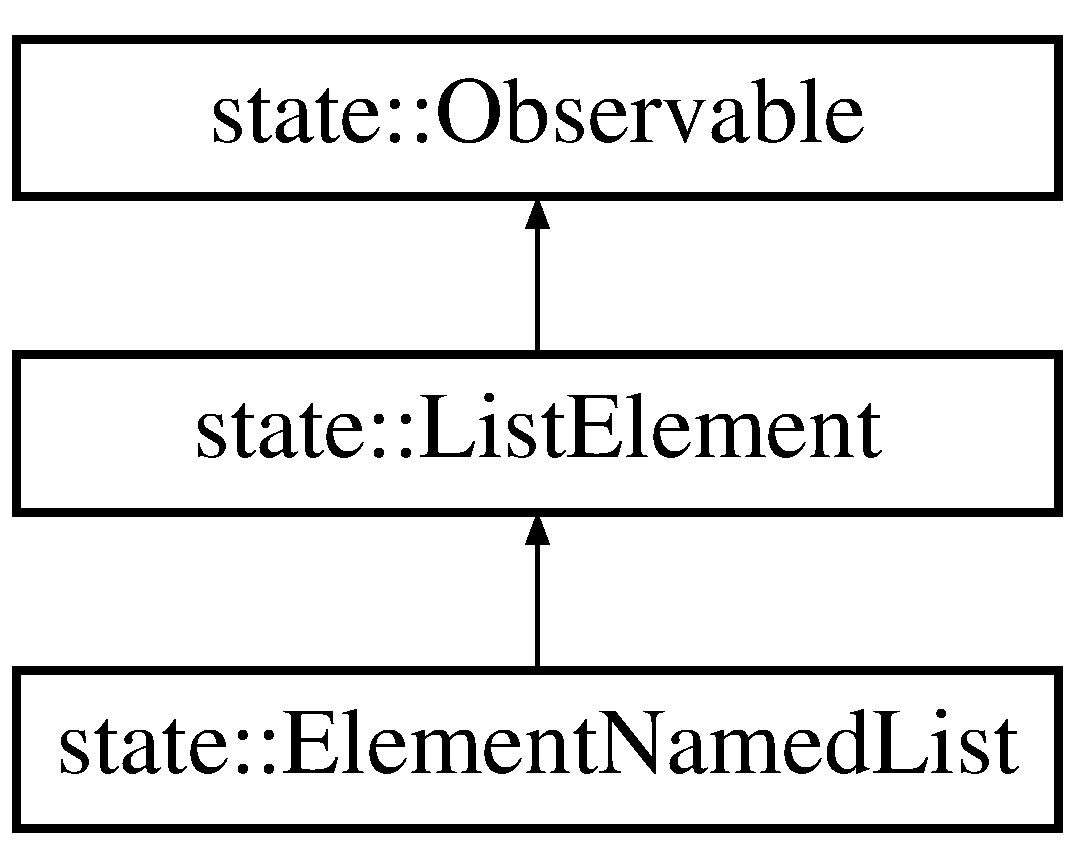
\includegraphics[height=3.000000cm]{classstate_1_1_element_named_list}
\end{center}
\end{figure}
\subsection*{Public Member Functions}
\begin{DoxyCompactItemize}
\item 
\hyperlink{classstate_1_1_element_named_list_a233b7af7b1421ef71f562746a068049f}{Element\+Named\+List} (List\+Type name)
\item 
virtual \hyperlink{classstate_1_1_element_named_list_acbc647aa8ded664094ffbc47ab14178b}{$\sim$\+Element\+Named\+List} ()
\item 
List\+Type \hyperlink{classstate_1_1_element_named_list_a7a85fde8e5274020221ef1f521b9d2ea}{Getname} ()
\item 
void \hyperlink{classstate_1_1_element_named_list_a8f16293821685af35edfc3f77be55a5f}{update\+Pos} ()
\item 
bool \hyperlink{classstate_1_1_element_named_list_aa343185b2217042714b7020320166da9}{add} (\hyperlink{classstate_1_1_element}{Element} $\ast$e)
\item 
bool \hyperlink{classstate_1_1_element_named_list_a96b53623f9c61dd9867718b87f20ff03}{suppr} (int idx)
\item 
\hyperlink{classstate_1_1_element}{Element} $\ast$ \hyperlink{classstate_1_1_element_named_list_acd3748ad2d2f1d593f0c79508f067641}{is\+Here} (int x, int y)
\end{DoxyCompactItemize}
\subsection*{Additional Inherited Members}


\subsection{Constructor \& Destructor Documentation}
\mbox{\Hypertarget{classstate_1_1_element_named_list_a233b7af7b1421ef71f562746a068049f}\label{classstate_1_1_element_named_list_a233b7af7b1421ef71f562746a068049f}} 
\index{state\+::\+Element\+Named\+List@{state\+::\+Element\+Named\+List}!Element\+Named\+List@{Element\+Named\+List}}
\index{Element\+Named\+List@{Element\+Named\+List}!state\+::\+Element\+Named\+List@{state\+::\+Element\+Named\+List}}
\subsubsection{\texorpdfstring{Element\+Named\+List()}{ElementNamedList()}}
{\footnotesize\ttfamily state\+::\+Element\+Named\+List\+::\+Element\+Named\+List (\begin{DoxyParamCaption}\item[{List\+Type}]{name }\end{DoxyParamCaption})}

Default constructor \mbox{\Hypertarget{classstate_1_1_element_named_list_acbc647aa8ded664094ffbc47ab14178b}\label{classstate_1_1_element_named_list_acbc647aa8ded664094ffbc47ab14178b}} 
\index{state\+::\+Element\+Named\+List@{state\+::\+Element\+Named\+List}!````~Element\+Named\+List@{$\sim$\+Element\+Named\+List}}
\index{````~Element\+Named\+List@{$\sim$\+Element\+Named\+List}!state\+::\+Element\+Named\+List@{state\+::\+Element\+Named\+List}}
\subsubsection{\texorpdfstring{$\sim$\+Element\+Named\+List()}{~ElementNamedList()}}
{\footnotesize\ttfamily state\+::\+Element\+Named\+List\+::$\sim$\+Element\+Named\+List (\begin{DoxyParamCaption}{ }\end{DoxyParamCaption})\hspace{0.3cm}{\ttfamily [virtual]}}

Default destructor 

\subsection{Member Function Documentation}
\mbox{\Hypertarget{classstate_1_1_element_named_list_aa343185b2217042714b7020320166da9}\label{classstate_1_1_element_named_list_aa343185b2217042714b7020320166da9}} 
\index{state\+::\+Element\+Named\+List@{state\+::\+Element\+Named\+List}!add@{add}}
\index{add@{add}!state\+::\+Element\+Named\+List@{state\+::\+Element\+Named\+List}}
\subsubsection{\texorpdfstring{add()}{add()}}
{\footnotesize\ttfamily bool state\+::\+Element\+Named\+List\+::add (\begin{DoxyParamCaption}\item[{\hyperlink{classstate_1_1_element}{Element} $\ast$}]{e }\end{DoxyParamCaption})}

Ajouter un éléments à la liste \begin{DoxyReturn}{Returns}
True si l\textquotesingle{}élèments a bien été insérer 
\end{DoxyReturn}
\mbox{\Hypertarget{classstate_1_1_element_named_list_a7a85fde8e5274020221ef1f521b9d2ea}\label{classstate_1_1_element_named_list_a7a85fde8e5274020221ef1f521b9d2ea}} 
\index{state\+::\+Element\+Named\+List@{state\+::\+Element\+Named\+List}!Getname@{Getname}}
\index{Getname@{Getname}!state\+::\+Element\+Named\+List@{state\+::\+Element\+Named\+List}}
\subsubsection{\texorpdfstring{Getname()}{Getname()}}
{\footnotesize\ttfamily List\+Type state\+::\+Element\+Named\+List\+::\+Getname (\begin{DoxyParamCaption}{ }\end{DoxyParamCaption})\hspace{0.3cm}{\ttfamily [inline]}}

Access name \begin{DoxyReturn}{Returns}
The current value of name 
\end{DoxyReturn}
\mbox{\Hypertarget{classstate_1_1_element_named_list_acd3748ad2d2f1d593f0c79508f067641}\label{classstate_1_1_element_named_list_acd3748ad2d2f1d593f0c79508f067641}} 
\index{state\+::\+Element\+Named\+List@{state\+::\+Element\+Named\+List}!is\+Here@{is\+Here}}
\index{is\+Here@{is\+Here}!state\+::\+Element\+Named\+List@{state\+::\+Element\+Named\+List}}
\subsubsection{\texorpdfstring{is\+Here()}{isHere()}}
{\footnotesize\ttfamily \hyperlink{classstate_1_1_element}{Element} $\ast$ state\+::\+Element\+Named\+List\+::is\+Here (\begin{DoxyParamCaption}\item[{int}]{x,  }\item[{int}]{y }\end{DoxyParamCaption})}

Trouver un éléments par sa position \begin{DoxyReturn}{Returns}
L\textquotesingle{}élément a la position ou N\+U\+LL sinon 
\end{DoxyReturn}
\mbox{\Hypertarget{classstate_1_1_element_named_list_a96b53623f9c61dd9867718b87f20ff03}\label{classstate_1_1_element_named_list_a96b53623f9c61dd9867718b87f20ff03}} 
\index{state\+::\+Element\+Named\+List@{state\+::\+Element\+Named\+List}!suppr@{suppr}}
\index{suppr@{suppr}!state\+::\+Element\+Named\+List@{state\+::\+Element\+Named\+List}}
\subsubsection{\texorpdfstring{suppr()}{suppr()}}
{\footnotesize\ttfamily bool state\+::\+Element\+Named\+List\+::suppr (\begin{DoxyParamCaption}\item[{int}]{idx }\end{DoxyParamCaption})}

Delete un élèments de la liste \begin{DoxyReturn}{Returns}
True si l\textquotesingle{}éléments a bien été supprimer (index valide) 
\end{DoxyReturn}
\mbox{\Hypertarget{classstate_1_1_element_named_list_a8f16293821685af35edfc3f77be55a5f}\label{classstate_1_1_element_named_list_a8f16293821685af35edfc3f77be55a5f}} 
\index{state\+::\+Element\+Named\+List@{state\+::\+Element\+Named\+List}!update\+Pos@{update\+Pos}}
\index{update\+Pos@{update\+Pos}!state\+::\+Element\+Named\+List@{state\+::\+Element\+Named\+List}}
\subsubsection{\texorpdfstring{update\+Pos()}{updatePos()}}
{\footnotesize\ttfamily void state\+::\+Element\+Named\+List\+::update\+Pos (\begin{DoxyParamCaption}{ }\end{DoxyParamCaption})}

Update animation \begin{DoxyReturn}{Returns}
No return 
\end{DoxyReturn}
To do 

The documentation for this class was generated from the following files\+:\begin{DoxyCompactItemize}
\item 
C\+:/\+Users/corentin/\+Desktop/projet tank/src modif/\+Tank\+State/include/Element\+Named\+List.\+h\item 
C\+:/\+Users/corentin/\+Desktop/projet tank/src modif/\+Tank\+State/src/Element\+Named\+List.\+cpp\end{DoxyCompactItemize}

\hypertarget{classstate_1_1_global_state}{}\section{state\+:\+:Global\+State Class Reference}
\label{classstate_1_1_global_state}\index{state\+::\+Global\+State@{state\+::\+Global\+State}}


class State -\/ Store the list of the elements of the background (grid) and the list of the tank(mobiles)  




{\ttfamily \#include $<$Global\+State.\+h$>$}

Inheritance diagram for state\+:\+:Global\+State\+:\begin{figure}[H]
\begin{center}
\leavevmode
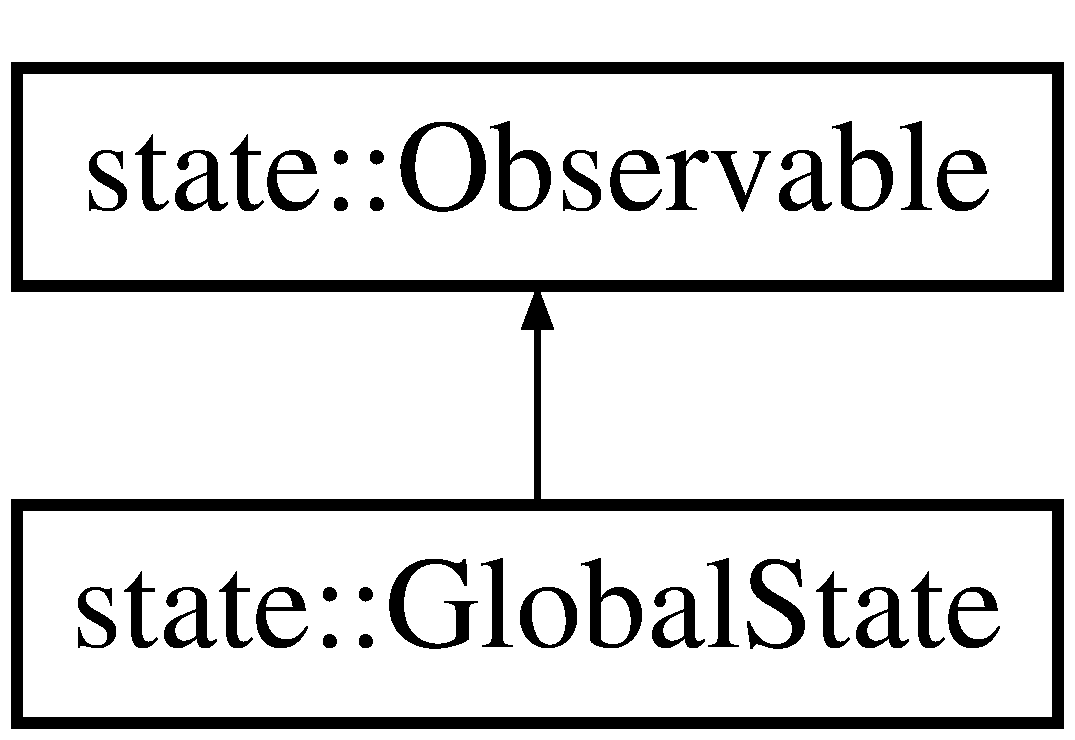
\includegraphics[height=2.000000cm]{classstate_1_1_global_state}
\end{center}
\end{figure}
\subsection*{Public Member Functions}
\begin{DoxyCompactItemize}
\item 
\mbox{\Hypertarget{classstate_1_1_global_state_aafb29e5a90ae4f8e27d25ed3c186dd80}\label{classstate_1_1_global_state_aafb29e5a90ae4f8e27d25ed3c186dd80}} 
\hyperlink{classstate_1_1_global_state_aafb29e5a90ae4f8e27d25ed3c186dd80}{Global\+State} ()
\begin{DoxyCompactList}\small\item\em class State -\/ mobiles-\/$>$ liste des truc mobile (tank, missile) \end{DoxyCompactList}\item 
\mbox{\Hypertarget{classstate_1_1_global_state_a9d868ea2e34692ccbc1fd648bbbc7eea}\label{classstate_1_1_global_state_a9d868ea2e34692ccbc1fd648bbbc7eea}} 
\hyperlink{classstate_1_1_element_grid}{Element\+Grid} \& {\bfseries get\+Grid} ()
\item 
\mbox{\Hypertarget{classstate_1_1_global_state_a41e3ba4093579173405af0ca54c0f06d}\label{classstate_1_1_global_state_a41e3ba4093579173405af0ca54c0f06d}} 
const \hyperlink{classstate_1_1_element_grid}{Element\+Grid} \& {\bfseries get\+Grid} () const
\item 
\mbox{\Hypertarget{classstate_1_1_global_state_abe00dc79287ea41a01127ae580b720f4}\label{classstate_1_1_global_state_abe00dc79287ea41a01127ae580b720f4}} 
\hyperlink{classstate_1_1_list_element}{List\+Element} \& {\bfseries get\+Mobiles} ()
\item 
\mbox{\Hypertarget{classstate_1_1_global_state_a77b88d9885aba43976ec8eab9ef7db64}\label{classstate_1_1_global_state_a77b88d9885aba43976ec8eab9ef7db64}} 
const \hyperlink{classstate_1_1_list_element}{List\+Element} \& {\bfseries get\+Mobiles} () const
\item 
\mbox{\Hypertarget{classstate_1_1_global_state_a2f2626fa22999e1d45d2fb82f5142f9f}\label{classstate_1_1_global_state_a2f2626fa22999e1d45d2fb82f5142f9f}} 
\hyperlink{classstate_1_1_element}{Element} $\ast$ {\bfseries get\+Mobile} (int idx)
\item 
\mbox{\Hypertarget{classstate_1_1_global_state_ac6fc2db0c360c6014fb161062b882679}\label{classstate_1_1_global_state_ac6fc2db0c360c6014fb161062b882679}} 
const \hyperlink{classstate_1_1_element}{Element} $\ast$ {\bfseries get\+Mobile} (int idx) const
\item 
\mbox{\Hypertarget{classstate_1_1_global_state_aec97fdccde7f2733b799b328375bdf81}\label{classstate_1_1_global_state_aec97fdccde7f2733b799b328375bdf81}} 
void {\bfseries load} (const char $\ast$file\+\_\+name)
\item 
\mbox{\Hypertarget{classstate_1_1_global_state_a91c7898318ef25c9a3481a9863fd9c21}\label{classstate_1_1_global_state_a91c7898318ef25c9a3481a9863fd9c21}} 
void {\bfseries notify\+Observer} (const \hyperlink{classstate_1_1_state_event}{State\+Event} \&event) const
\item 
\mbox{\Hypertarget{classstate_1_1_global_state_abd600cd6bf17f0f2046d8af0c604b35f}\label{classstate_1_1_global_state_abd600cd6bf17f0f2046d8af0c604b35f}} 
void {\bfseries copy} (const \hyperlink{classstate_1_1_global_state}{Global\+State} s)
\end{DoxyCompactItemize}
\subsection*{Protected Attributes}
\begin{DoxyCompactItemize}
\item 
\mbox{\Hypertarget{classstate_1_1_global_state_a483c8cbfeb541e31b6aa486eb994b74f}\label{classstate_1_1_global_state_a483c8cbfeb541e31b6aa486eb994b74f}} 
\hyperlink{classstate_1_1_list_element}{List\+Element} {\bfseries mobiles}
\item 
\mbox{\Hypertarget{classstate_1_1_global_state_a637c91d09cfc38a64ef28ce79c2a8927}\label{classstate_1_1_global_state_a637c91d09cfc38a64ef28ce79c2a8927}} 
\hyperlink{classstate_1_1_element_grid}{Element\+Grid} {\bfseries grid}
\end{DoxyCompactItemize}


\subsection{Detailed Description}
class State -\/ Store the list of the elements of the background (grid) and the list of the tank(mobiles) 

The documentation for this class was generated from the following files\+:\begin{DoxyCompactItemize}
\item 
C\+:/\+Users/corentin/\+Desktop/projet tank/src modif/\+Tank\+State/include/Global\+State.\+h\item 
C\+:/\+Users/corentin/\+Desktop/projet tank/src modif/\+Tank\+State/src/Global\+State.\+cpp\end{DoxyCompactItemize}

\hypertarget{classstate_1_1_list_element}{}\section{state\+:\+:List\+Element Class Reference}
\label{classstate_1_1_list_element}\index{state\+::\+List\+Element@{state\+::\+List\+Element}}


class \hyperlink{classstate_1_1_element_list}{Element\+List} -\/ List of Elements  




{\ttfamily \#include $<$List\+Element.\+h$>$}

Inheritance diagram for state\+:\+:List\+Element\+:\begin{figure}[H]
\begin{center}
\leavevmode
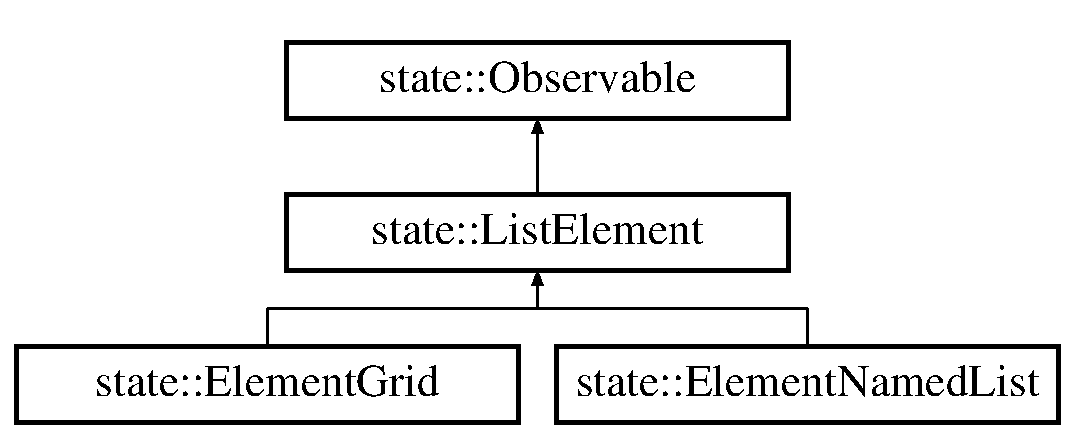
\includegraphics[height=3.000000cm]{classstate_1_1_list_element}
\end{center}
\end{figure}
\subsection*{Public Member Functions}
\begin{DoxyCompactItemize}
\item 
\mbox{\Hypertarget{classstate_1_1_list_element_a1471bc2a449803cfd9932ed15f153654}\label{classstate_1_1_list_element_a1471bc2a449803cfd9932ed15f153654}} 
\hyperlink{classstate_1_1_list_element_a1471bc2a449803cfd9932ed15f153654}{List\+Element} ()
\begin{DoxyCompactList}\small\item\em class \hyperlink{classstate_1_1_list_element}{List\+Element} -\/ c \end{DoxyCompactList}\item 
\mbox{\Hypertarget{classstate_1_1_list_element_a70fef2b8268f830bdf7295d4c05c422c}\label{classstate_1_1_list_element_a70fef2b8268f830bdf7295d4c05c422c}} 
int {\bfseries size} () const
\item 
\mbox{\Hypertarget{classstate_1_1_list_element_a514900215f7548c74e2f3290ff5e4d1c}\label{classstate_1_1_list_element_a514900215f7548c74e2f3290ff5e4d1c}} 
\hyperlink{classstate_1_1_element}{Element} $\ast$ {\bfseries get} (int idx) const
\item 
\mbox{\Hypertarget{classstate_1_1_list_element_ab7b04acd17cd9281f269b24e43a202ed}\label{classstate_1_1_list_element_ab7b04acd17cd9281f269b24e43a202ed}} 
void {\bfseries clear} ()
\item 
\mbox{\Hypertarget{classstate_1_1_list_element_af9d588bb5d6c19a90a997d03d2fc538f}\label{classstate_1_1_list_element_af9d588bb5d6c19a90a997d03d2fc538f}} 
void {\bfseries set} (int idx, \hyperlink{classstate_1_1_element}{Element} $\ast$e)
\item 
\mbox{\Hypertarget{classstate_1_1_list_element_a5a6f3a66e07bfca10a817d2b55702f16}\label{classstate_1_1_list_element_a5a6f3a66e07bfca10a817d2b55702f16}} 
void {\bfseries load} (const char $\ast$path)
\item 
\mbox{\Hypertarget{classstate_1_1_list_element_a2ea8ec069e8691d7d3300792091280a8}\label{classstate_1_1_list_element_a2ea8ec069e8691d7d3300792091280a8}} 
void {\bfseries notify\+Observer} (int idx=-\/1) const
\item 
\mbox{\Hypertarget{classstate_1_1_list_element_ae60d45d8fab384b8ad942dc337ee273e}\label{classstate_1_1_list_element_ae60d45d8fab384b8ad942dc337ee273e}} 
void {\bfseries notify\+Observer} (const \hyperlink{classstate_1_1_state_event}{State\+Event} \&event) const
\item 
\mbox{\Hypertarget{classstate_1_1_list_element_a00524c983fc53699699e9ff5929103e7}\label{classstate_1_1_list_element_a00524c983fc53699699e9ff5929103e7}} 
virtual void {\bfseries copy} (const \hyperlink{classstate_1_1_list_element}{List\+Element} e)
\end{DoxyCompactItemize}
\subsection*{Protected Attributes}
\begin{DoxyCompactItemize}
\item 
\mbox{\Hypertarget{classstate_1_1_list_element_ad7d70434d4cd8450466d6e4a094b1ac3}\label{classstate_1_1_list_element_ad7d70434d4cd8450466d6e4a094b1ac3}} 
std\+::vector$<$ \hyperlink{classstate_1_1_element}{Element} $\ast$ $>$ {\bfseries elements}
\end{DoxyCompactItemize}


\subsection{Detailed Description}
class \hyperlink{classstate_1_1_element_list}{Element\+List} -\/ List of Elements 

The documentation for this class was generated from the following files\+:\begin{DoxyCompactItemize}
\item 
C\+:/\+Users/corentin/\+Desktop/projet tank/src modif/\+Tank\+State/include/List\+Element.\+h\item 
C\+:/\+Users/corentin/\+Desktop/projet tank/src modif/\+Tank\+State/src/List\+Element.\+cpp\end{DoxyCompactItemize}

\hypertarget{classstate_1_1_observable}{}\section{state\+:\+:Observable Class Reference}
\label{classstate_1_1_observable}\index{state\+::\+Observable@{state\+::\+Observable}}


class \hyperlink{classstate_1_1_observable}{Observable} -\/ List of the class\textquotesingle{}s observers  




{\ttfamily \#include $<$Observable.\+h$>$}

Inheritance diagram for state\+:\+:Observable\+:\begin{figure}[H]
\begin{center}
\leavevmode
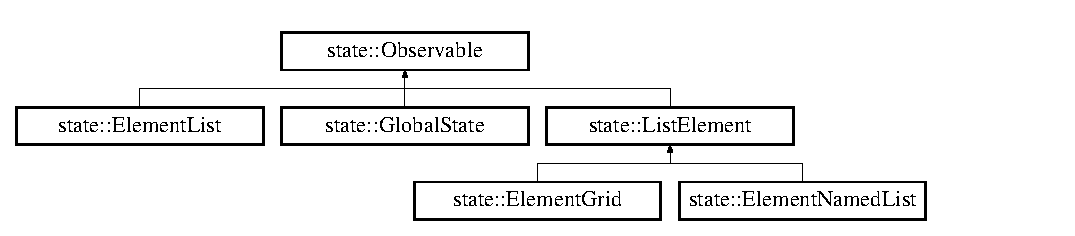
\includegraphics[height=2.727273cm]{classstate_1_1_observable}
\end{center}
\end{figure}
\subsection*{Public Member Functions}
\begin{DoxyCompactItemize}
\item 
\mbox{\Hypertarget{classstate_1_1_observable_a3be8c3715d705eb217abbd5c80718ce7}\label{classstate_1_1_observable_a3be8c3715d705eb217abbd5c80718ce7}} 
void {\bfseries register\+Observer} (\hyperlink{classstate_1_1_state_observer}{State\+Observer} $\ast$obs) const
\item 
\mbox{\Hypertarget{classstate_1_1_observable_ab7c1dc9dc8f731d89f0285a993bc20d9}\label{classstate_1_1_observable_ab7c1dc9dc8f731d89f0285a993bc20d9}} 
virtual void {\bfseries notify\+Observer} (const \hyperlink{classstate_1_1_state_event}{State\+Event} \&event) const
\end{DoxyCompactItemize}
\subsection*{Protected Attributes}
\begin{DoxyCompactItemize}
\item 
\mbox{\Hypertarget{classstate_1_1_observable_afbb99906de5c948b84026cdf0cf154b3}\label{classstate_1_1_observable_afbb99906de5c948b84026cdf0cf154b3}} 
std\+::vector$<$ \hyperlink{classstate_1_1_state_observer}{State\+Observer} $\ast$ $>$ {\bfseries observers}
\end{DoxyCompactItemize}


\subsection{Detailed Description}
class \hyperlink{classstate_1_1_observable}{Observable} -\/ List of the class\textquotesingle{}s observers 

The documentation for this class was generated from the following files\+:\begin{DoxyCompactItemize}
\item 
C\+:/\+Users/corentin/\+Desktop/projet tank/src modif/\+Tank\+State/include/Observable.\+h\item 
C\+:/\+Users/corentin/\+Desktop/projet tank/src modif/\+Tank\+State/src/Observable.\+cpp\end{DoxyCompactItemize}

\hypertarget{classstate_1_1_obstacle}{}\section{state\+:\+:Obstacle Class Reference}
\label{classstate_1_1_obstacle}\index{state\+::\+Obstacle@{state\+::\+Obstacle}}


class \hyperlink{classstate_1_1_obstacle}{Obstacle} -\/  




{\ttfamily \#include $<$Obstacle.\+h$>$}

Inheritance diagram for state\+:\+:Obstacle\+:\begin{figure}[H]
\begin{center}
\leavevmode
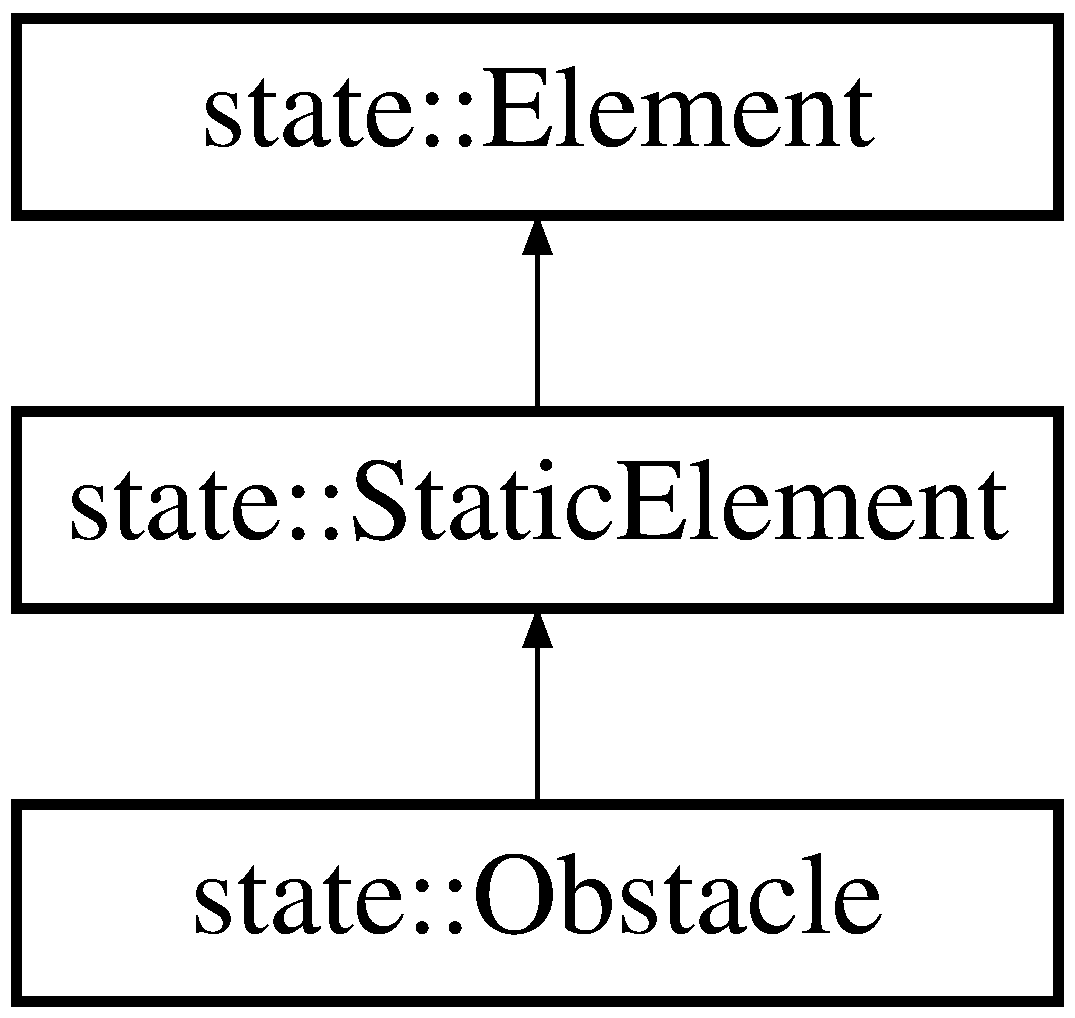
\includegraphics[height=3.000000cm]{classstate_1_1_obstacle}
\end{center}
\end{figure}
\subsection*{Public Member Functions}
\begin{DoxyCompactItemize}
\item 
\mbox{\Hypertarget{classstate_1_1_obstacle_a81d2e344286f1bedde13f90ef118379e}\label{classstate_1_1_obstacle_a81d2e344286f1bedde13f90ef118379e}} 
{\bfseries Obstacle} (Obstacle\+Type\+Id id, int x, int y)
\item 
\mbox{\Hypertarget{classstate_1_1_obstacle_a4d0fe501eb6d1227b889db3845cada77}\label{classstate_1_1_obstacle_a4d0fe501eb6d1227b889db3845cada77}} 
virtual bool {\bfseries is\+Space} () const
\item 
\mbox{\Hypertarget{classstate_1_1_obstacle_acae46baf30f68bd3c9a8f3dd3ba347c7}\label{classstate_1_1_obstacle_acae46baf30f68bd3c9a8f3dd3ba347c7}} 
Type\+Id {\bfseries get\+Type\+Id} () const
\item 
\mbox{\Hypertarget{classstate_1_1_obstacle_ab3e90122c3e034912c072a30a99fc483}\label{classstate_1_1_obstacle_ab3e90122c3e034912c072a30a99fc483}} 
void {\bfseries set\+Obstacle\+Type\+Id} (Obstacle\+Type\+Id id)
\item 
\mbox{\Hypertarget{classstate_1_1_obstacle_addedbd209e4690453db32de2e8ca95a7}\label{classstate_1_1_obstacle_addedbd209e4690453db32de2e8ca95a7}} 
Obstacle\+Type\+Id {\bfseries get\+Obstacle\+Type\+Id} () const
\item 
\mbox{\Hypertarget{classstate_1_1_obstacle_aedae2b6e04a1782212513bbb6eaf953d}\label{classstate_1_1_obstacle_aedae2b6e04a1782212513bbb6eaf953d}} 
\hyperlink{classstate_1_1_element}{Element} $\ast$ {\bfseries clone} () const
\end{DoxyCompactItemize}
\subsection*{Additional Inherited Members}


\subsection{Detailed Description}
class \hyperlink{classstate_1_1_obstacle}{Obstacle} -\/ 

The documentation for this class was generated from the following files\+:\begin{DoxyCompactItemize}
\item 
C\+:/\+Users/corentin/\+Desktop/projet tank/src modif/\+Tank\+State/include/Obstacle.\+h\item 
C\+:/\+Users/corentin/\+Desktop/projet tank/src modif/\+Tank\+State/src/Obstacle.\+cpp\end{DoxyCompactItemize}

\hypertarget{class_projectile}{}\section{Projectile Class Reference}
\label{class_projectile}\index{Projectile@{Projectile}}
Inheritance diagram for Projectile\+:\begin{figure}[H]
\begin{center}
\leavevmode
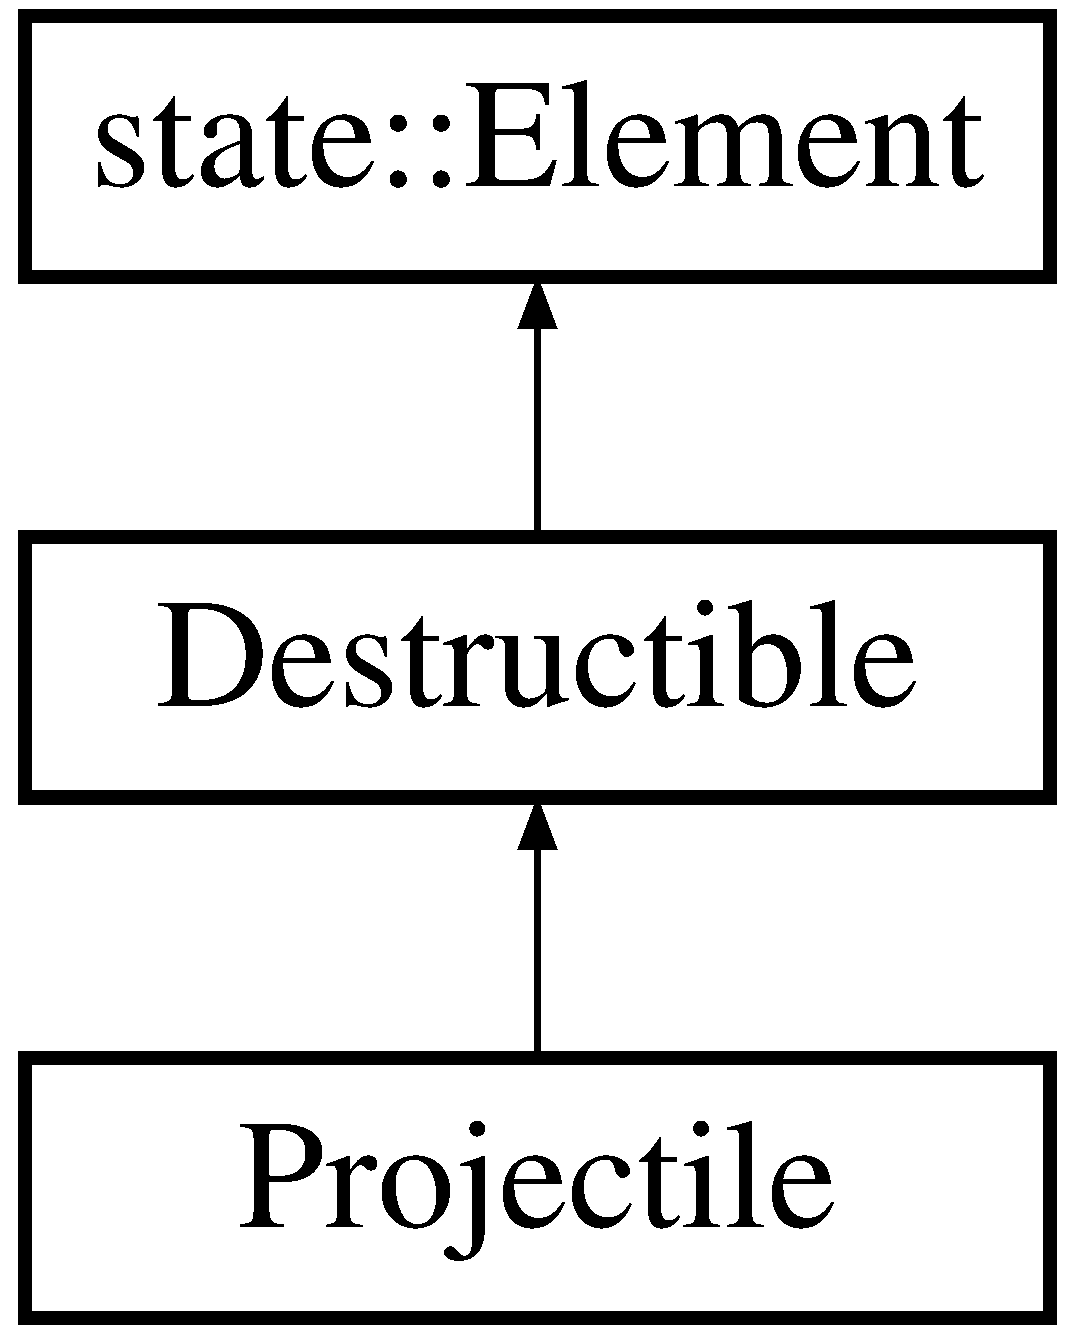
\includegraphics[height=3.000000cm]{class_projectile}
\end{center}
\end{figure}
\subsection*{Public Member Functions}
\begin{DoxyCompactItemize}
\item 
\mbox{\Hypertarget{class_projectile_a7c76e234b9424374db802d83901cc9c0}\label{class_projectile_a7c76e234b9424374db802d83901cc9c0}} 
{\bfseries Projectile} (int x, int y)
\item 
bool \hyperlink{class_projectile_ab667833975b19a5b1a5ab6c3722da3dd}{update\+Position} ()
\item 
\mbox{\Hypertarget{class_projectile_a7a4c33abdde47e2cefaeb64f9b7a5492}\label{class_projectile_a7a4c33abdde47e2cefaeb64f9b7a5492}} 
void \hyperlink{class_projectile_a7a4c33abdde47e2cefaeb64f9b7a5492}{Setvitesse} (int val)
\begin{DoxyCompactList}\small\item\em Getteur. \end{DoxyCompactList}\item 
\mbox{\Hypertarget{class_projectile_a31c436c8b15f0f5c183db1f97835fea1}\label{class_projectile_a31c436c8b15f0f5c183db1f97835fea1}} 
void {\bfseries Setdirection} (int val)
\item 
\mbox{\Hypertarget{class_projectile_a97eef85a7cb2e20ec2e65a3321cfeac0}\label{class_projectile_a97eef85a7cb2e20ec2e65a3321cfeac0}} 
void {\bfseries Setpath\+Type} (int val)
\item 
\mbox{\Hypertarget{class_projectile_ab7695bd05ed63e7ceeb96e6aed3d6a28}\label{class_projectile_ab7695bd05ed63e7ceeb96e6aed3d6a28}} 
void {\bfseries Setdegat} (int val)
\end{DoxyCompactItemize}
\subsection*{Additional Inherited Members}


\subsection{Member Function Documentation}
\mbox{\Hypertarget{class_projectile_ab667833975b19a5b1a5ab6c3722da3dd}\label{class_projectile_ab667833975b19a5b1a5ab6c3722da3dd}} 
\index{Projectile@{Projectile}!update\+Position@{update\+Position}}
\index{update\+Position@{update\+Position}!Projectile@{Projectile}}
\subsubsection{\texorpdfstring{update\+Position()}{updatePosition()}}
{\footnotesize\ttfamily bool Projectile\+::update\+Position (\begin{DoxyParamCaption}{ }\end{DoxyParamCaption})}

formule de calcul a mettre 

The documentation for this class was generated from the following files\+:\begin{DoxyCompactItemize}
\item 
C\+:/\+Users/corentin/\+Desktop/projet tank/src modif/\+Tank\+State/include/Projectile.\+h\item 
C\+:/\+Users/corentin/\+Desktop/projet tank/src modif/\+Tank\+State/src/Projectile.\+cpp\end{DoxyCompactItemize}

\hypertarget{classstate_1_1_projectile_event}{}\section{state\+:\+:Projectile\+Event Class Reference}
\label{classstate_1_1_projectile_event}\index{state\+::\+Projectile\+Event@{state\+::\+Projectile\+Event}}


class \hyperlink{classstate_1_1_projectile_event}{Projectile\+Event} -\/ Event \char`\"{}\+Projectile\+\_\+\+Event\char`\"{}  




{\ttfamily \#include $<$Projectile\+Event.\+h$>$}

Inheritance diagram for state\+:\+:Projectile\+Event\+:\begin{figure}[H]
\begin{center}
\leavevmode
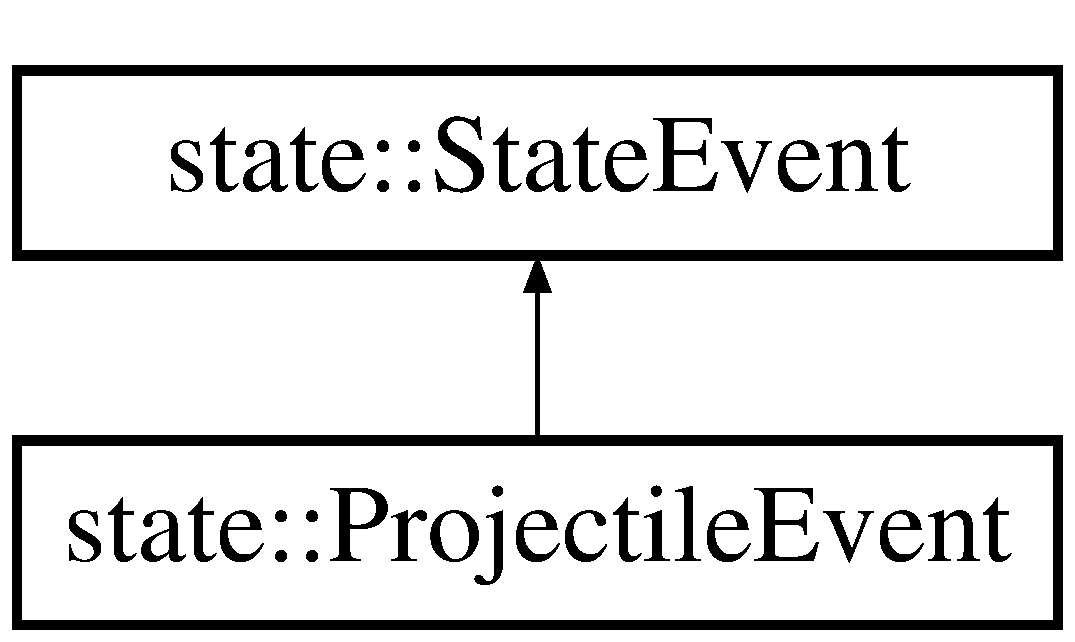
\includegraphics[height=2.000000cm]{classstate_1_1_projectile_event}
\end{center}
\end{figure}
\subsection*{Public Member Functions}
\begin{DoxyCompactItemize}
\item 
\mbox{\Hypertarget{classstate_1_1_projectile_event_ac928f6136bc7d2b665bd8c6c14494fd4}\label{classstate_1_1_projectile_event_ac928f6136bc7d2b665bd8c6c14494fd4}} 
{\bfseries Projectile\+Event} (int x\+Start, int y\+Start, int x\+Impact, int y\+Impact, bool right\+Direction=true, int y\+Max=-\/1)
\item 
\mbox{\Hypertarget{classstate_1_1_projectile_event_aade858440992f7404e9a6b82ed18fb11}\label{classstate_1_1_projectile_event_aade858440992f7404e9a6b82ed18fb11}} 
\hyperlink{classstate_1_1_state_event}{State\+Event} $\ast$ {\bfseries clone} () const
\end{DoxyCompactItemize}
\subsection*{Public Attributes}
\begin{DoxyCompactItemize}
\item 
\mbox{\Hypertarget{classstate_1_1_projectile_event_ab931a89ed170f9222d643f3713738cf1}\label{classstate_1_1_projectile_event_ab931a89ed170f9222d643f3713738cf1}} 
int {\bfseries x\+Start}
\item 
\mbox{\Hypertarget{classstate_1_1_projectile_event_aed1874d2894fcc6629eaa07f569416b2}\label{classstate_1_1_projectile_event_aed1874d2894fcc6629eaa07f569416b2}} 
int {\bfseries y\+Start}
\item 
\mbox{\Hypertarget{classstate_1_1_projectile_event_a0ba25dfd2661474f0fdbdd4a6a201efa}\label{classstate_1_1_projectile_event_a0ba25dfd2661474f0fdbdd4a6a201efa}} 
int {\bfseries x\+Impact}
\item 
\mbox{\Hypertarget{classstate_1_1_projectile_event_af7d792e2b10cba7ab4e70eefb2208217}\label{classstate_1_1_projectile_event_af7d792e2b10cba7ab4e70eefb2208217}} 
int {\bfseries y\+Impact}
\item 
\mbox{\Hypertarget{classstate_1_1_projectile_event_a83b5a7e8e24361cfcebb5496008424bc}\label{classstate_1_1_projectile_event_a83b5a7e8e24361cfcebb5496008424bc}} 
int {\bfseries y\+Max}
\item 
\mbox{\Hypertarget{classstate_1_1_projectile_event_a641c54c8c1bda4cae0e4547b4c2a1d4a}\label{classstate_1_1_projectile_event_a641c54c8c1bda4cae0e4547b4c2a1d4a}} 
bool {\bfseries right\+Direction}
\end{DoxyCompactItemize}


\subsection{Detailed Description}
class \hyperlink{classstate_1_1_projectile_event}{Projectile\+Event} -\/ Event \char`\"{}\+Projectile\+\_\+\+Event\char`\"{} 

The documentation for this class was generated from the following files\+:\begin{DoxyCompactItemize}
\item 
C\+:/\+Users/corentin/\+Desktop/projet tank/src modif/\+Tank\+State/include/Projectile\+Event.\+h\item 
C\+:/\+Users/corentin/\+Desktop/projet tank/src modif/\+Tank\+State/src/Projectile\+Event.\+cpp\end{DoxyCompactItemize}

\hypertarget{classstate_1_1_space}{}\section{state\+:\+:Space Class Reference}
\label{classstate_1_1_space}\index{state\+::\+Space@{state\+::\+Space}}


classe representant les elements traversable  




{\ttfamily \#include $<$Space.\+h$>$}

Inheritance diagram for state\+:\+:Space\+:\begin{figure}[H]
\begin{center}
\leavevmode
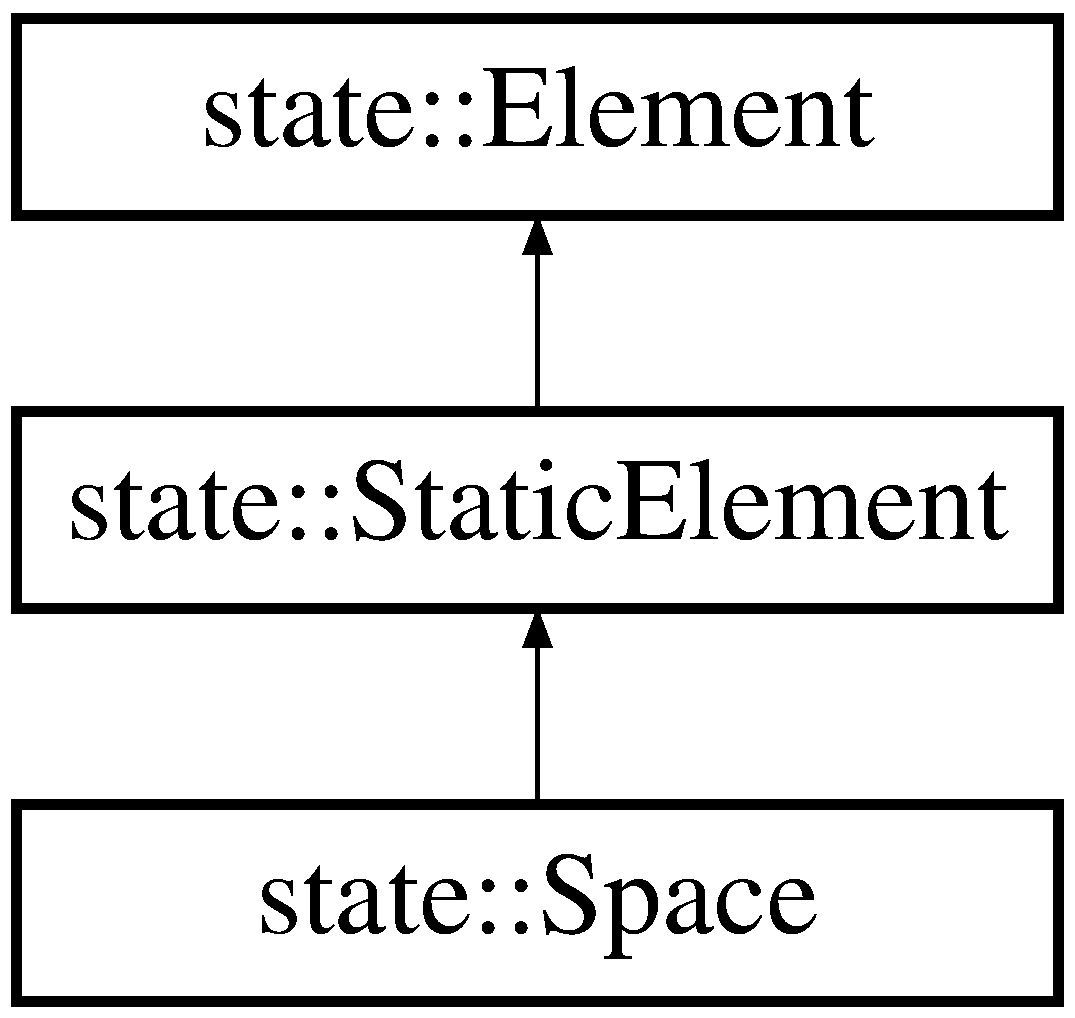
\includegraphics[height=3.000000cm]{classstate_1_1_space}
\end{center}
\end{figure}
\subsection*{Public Member Functions}
\begin{DoxyCompactItemize}
\item 
\hyperlink{classstate_1_1_space_a21cdd497cf2141748a05a30062ae2c4a}{Space} (Space\+Type\+Id id, int x, int y)
\begin{DoxyCompactList}\small\item\em A Constructor ; Crée un \hyperlink{classstate_1_1_space}{Space} de type id situé en (x,y) \end{DoxyCompactList}\item 
virtual bool \hyperlink{classstate_1_1_space_ae6a875b398ebe11adca364c5dc8a94a9}{is\+Space} () const
\begin{DoxyCompactList}\small\item\em Permet de determiner si l\textquotesingle{}éléments est un \hyperlink{classstate_1_1_space}{Space}. \end{DoxyCompactList}\item 
Type\+Id \hyperlink{classstate_1_1_space_a07fcfd9de95acfebb26e66f24f4ef519}{get\+Type\+Id} () const
\begin{DoxyCompactList}\small\item\em Permet de determiner le type d\textquotesingle{}élèment. \end{DoxyCompactList}\item 
Space\+Type\+Id \hyperlink{classstate_1_1_space_af05208d104c93dbffdb2643e2e2f54cf}{get\+Space\+Type\+Id} () const
\begin{DoxyCompactList}\small\item\em Permet de determiner l\textquotesingle{}aspect graphique de l\textquotesingle{}élèments. \end{DoxyCompactList}\item 
\hyperlink{classstate_1_1_element}{Element} $\ast$ \hyperlink{classstate_1_1_space_a2259b287265855ae2fee5050c4e4f97d}{clone} () const
\begin{DoxyCompactList}\small\item\em Fonction pour cloner l\textquotesingle{}élèment. \end{DoxyCompactList}\end{DoxyCompactItemize}
\subsection*{Additional Inherited Members}


\subsection{Detailed Description}
classe representant les elements traversable 

La classe gére les élèments traversable en leurs fournissant un aspect graphique et une position 

\subsection{Constructor \& Destructor Documentation}
\mbox{\Hypertarget{classstate_1_1_space_a21cdd497cf2141748a05a30062ae2c4a}\label{classstate_1_1_space_a21cdd497cf2141748a05a30062ae2c4a}} 
\index{state\+::\+Space@{state\+::\+Space}!Space@{Space}}
\index{Space@{Space}!state\+::\+Space@{state\+::\+Space}}
\subsubsection{\texorpdfstring{Space()}{Space()}}
{\footnotesize\ttfamily state\+::\+Space\+::\+Space (\begin{DoxyParamCaption}\item[{Space\+Type\+Id}]{id,  }\item[{int}]{x,  }\item[{int}]{y }\end{DoxyParamCaption})}



A Constructor ; Crée un \hyperlink{classstate_1_1_space}{Space} de type id situé en (x,y) 

class \hyperlink{classstate_1_1_space}{Space} -\/


\begin{DoxyParams}{Parameters}
{\em id} & \+: L\textquotesingle{}aspect graphique du space à crée \\
\hline
{\em x} & \+: La position x de l\textquotesingle{}élèment \\
\hline
{\em y} & \+: La position y de l\textquotesingle{}élèment \\
\hline
\end{DoxyParams}
\begin{DoxyReturn}{Returns}
None 
\end{DoxyReturn}


\subsection{Member Function Documentation}
\mbox{\Hypertarget{classstate_1_1_space_a2259b287265855ae2fee5050c4e4f97d}\label{classstate_1_1_space_a2259b287265855ae2fee5050c4e4f97d}} 
\index{state\+::\+Space@{state\+::\+Space}!clone@{clone}}
\index{clone@{clone}!state\+::\+Space@{state\+::\+Space}}
\subsubsection{\texorpdfstring{clone()}{clone()}}
{\footnotesize\ttfamily \hyperlink{classstate_1_1_element}{Element} $\ast$ state\+::\+Space\+::clone (\begin{DoxyParamCaption}{ }\end{DoxyParamCaption}) const\hspace{0.3cm}{\ttfamily [virtual]}}



Fonction pour cloner l\textquotesingle{}élèment. 

\begin{DoxyReturn}{Returns}
Un pointeur vers une copie de l\textquotesingle{}élèment. 
\end{DoxyReturn}


Implements \hyperlink{classstate_1_1_element}{state\+::\+Element}.

\mbox{\Hypertarget{classstate_1_1_space_af05208d104c93dbffdb2643e2e2f54cf}\label{classstate_1_1_space_af05208d104c93dbffdb2643e2e2f54cf}} 
\index{state\+::\+Space@{state\+::\+Space}!get\+Space\+Type\+Id@{get\+Space\+Type\+Id}}
\index{get\+Space\+Type\+Id@{get\+Space\+Type\+Id}!state\+::\+Space@{state\+::\+Space}}
\subsubsection{\texorpdfstring{get\+Space\+Type\+Id()}{getSpaceTypeId()}}
{\footnotesize\ttfamily Space\+Type\+Id state\+::\+Space\+::get\+Space\+Type\+Id (\begin{DoxyParamCaption}{ }\end{DoxyParamCaption}) const}



Permet de determiner l\textquotesingle{}aspect graphique de l\textquotesingle{}élèments. 

\begin{DoxyReturn}{Returns}
Le type de space. Permet de récupérer le type d\textquotesingle{}espace de l\textquotesingle{}élèment, en vue d\textquotesingle{}un display. 
\end{DoxyReturn}
\mbox{\Hypertarget{classstate_1_1_space_a07fcfd9de95acfebb26e66f24f4ef519}\label{classstate_1_1_space_a07fcfd9de95acfebb26e66f24f4ef519}} 
\index{state\+::\+Space@{state\+::\+Space}!get\+Type\+Id@{get\+Type\+Id}}
\index{get\+Type\+Id@{get\+Type\+Id}!state\+::\+Space@{state\+::\+Space}}
\subsubsection{\texorpdfstring{get\+Type\+Id()}{getTypeId()}}
{\footnotesize\ttfamily Type\+Id state\+::\+Space\+::get\+Type\+Id (\begin{DoxyParamCaption}{ }\end{DoxyParamCaption}) const\hspace{0.3cm}{\ttfamily [virtual]}}



Permet de determiner le type d\textquotesingle{}élèment. 

\begin{DoxyReturn}{Returns}
Le type d\textquotesingle{}élèments, tel que symbolisé par un Type\+Id. Permet de récupérer le type d\textquotesingle{}élèment, en vue d\textquotesingle{}un cast et d\textquotesingle{}une utilisation en temps que tel. 
\end{DoxyReturn}


Implements \hyperlink{classstate_1_1_element}{state\+::\+Element}.

\mbox{\Hypertarget{classstate_1_1_space_ae6a875b398ebe11adca364c5dc8a94a9}\label{classstate_1_1_space_ae6a875b398ebe11adca364c5dc8a94a9}} 
\index{state\+::\+Space@{state\+::\+Space}!is\+Space@{is\+Space}}
\index{is\+Space@{is\+Space}!state\+::\+Space@{state\+::\+Space}}
\subsubsection{\texorpdfstring{is\+Space()}{isSpace()}}
{\footnotesize\ttfamily bool state\+::\+Space\+::is\+Space (\begin{DoxyParamCaption}{ }\end{DoxyParamCaption}) const\hspace{0.3cm}{\ttfamily [virtual]}}



Permet de determiner si l\textquotesingle{}éléments est un \hyperlink{classstate_1_1_space}{Space}. 

\begin{DoxyReturn}{Returns}
True 
\end{DoxyReturn}


Implements \hyperlink{classstate_1_1_static_element}{state\+::\+Static\+Element}.



The documentation for this class was generated from the following files\+:\begin{DoxyCompactItemize}
\item 
C\+:/\+Users/corentin/\+Desktop/projet tank/src modif/\+Tank\+State/include/Space.\+h\item 
C\+:/\+Users/corentin/\+Desktop/projet tank/src modif/\+Tank\+State/src/\hyperlink{_space_8cpp}{Space.\+cpp}\end{DoxyCompactItemize}

\hypertarget{classstate_1_1_state_event}{}\section{state\+:\+:State\+Event Class Reference}
\label{classstate_1_1_state_event}\index{state\+::\+State\+Event@{state\+::\+State\+Event}}


class \hyperlink{classstate_1_1_state_event}{State\+Event} -\/ Event concerning the state  




{\ttfamily \#include $<$State\+Event.\+h$>$}

Inheritance diagram for state\+:\+:State\+Event\+:\begin{figure}[H]
\begin{center}
\leavevmode
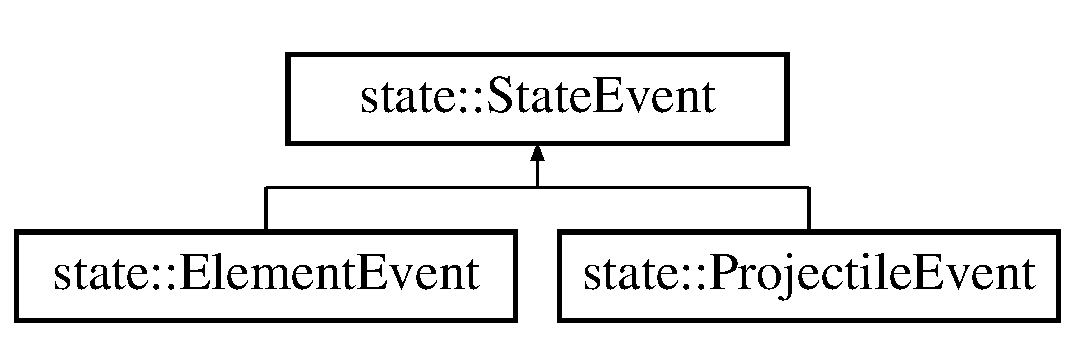
\includegraphics[height=2.000000cm]{classstate_1_1_state_event}
\end{center}
\end{figure}
\subsection*{Public Member Functions}
\begin{DoxyCompactItemize}
\item 
\mbox{\Hypertarget{classstate_1_1_state_event_aba4c5ef79ab8d4f7d4e3981221832d41}\label{classstate_1_1_state_event_aba4c5ef79ab8d4f7d4e3981221832d41}} 
{\bfseries State\+Event} (const \hyperlink{classstate_1_1_global_state}{Global\+State} $\ast$s, State\+Event\+Id id)
\item 
\mbox{\Hypertarget{classstate_1_1_state_event_a8c090eaaf0faf9bea8a38c257a813a39}\label{classstate_1_1_state_event_a8c090eaaf0faf9bea8a38c257a813a39}} 
bool {\bfseries operator==} (State\+Event\+Id id) const
\item 
\mbox{\Hypertarget{classstate_1_1_state_event_a89cb7184a64287e838e49c41b0b48bd5}\label{classstate_1_1_state_event_a89cb7184a64287e838e49c41b0b48bd5}} 
bool {\bfseries operator!=} (State\+Event\+Id id) const
\item 
\mbox{\Hypertarget{classstate_1_1_state_event_ae4bc562dbc81c2880ed3dd0f5dc83638}\label{classstate_1_1_state_event_ae4bc562dbc81c2880ed3dd0f5dc83638}} 
virtual \hyperlink{classstate_1_1_state_event}{State\+Event} $\ast$ {\bfseries clone} () const
\end{DoxyCompactItemize}
\subsection*{Public Attributes}
\begin{DoxyCompactItemize}
\item 
\mbox{\Hypertarget{classstate_1_1_state_event_abf29a1b9a3e094a064969faf9107e6c8}\label{classstate_1_1_state_event_abf29a1b9a3e094a064969faf9107e6c8}} 
const \hyperlink{classstate_1_1_global_state}{Global\+State} $\ast$ {\bfseries s}
\end{DoxyCompactItemize}


\subsection{Detailed Description}
class \hyperlink{classstate_1_1_state_event}{State\+Event} -\/ Event concerning the state 

The documentation for this class was generated from the following files\+:\begin{DoxyCompactItemize}
\item 
C\+:/\+Users/corentin/\+Desktop/projet tank/src modif/\+Tank\+State/include/State\+Event.\+h\item 
C\+:/\+Users/corentin/\+Desktop/projet tank/src modif/\+Tank\+State/src/State\+Event.\+cpp\end{DoxyCompactItemize}

\hypertarget{classstate_1_1_state_observer}{}\section{state\+:\+:State\+Observer Class Reference}
\label{classstate_1_1_state_observer}\index{state\+::\+State\+Observer@{state\+::\+State\+Observer}}


class \hyperlink{classstate_1_1_state_observer}{State\+Observer} -\/  




{\ttfamily \#include $<$State\+Observer.\+h$>$}

\subsection*{Public Member Functions}
\begin{DoxyCompactItemize}
\item 
\mbox{\Hypertarget{classstate_1_1_state_observer_a2e15f5d73a6e24786fbb40b22785cd99}\label{classstate_1_1_state_observer_a2e15f5d73a6e24786fbb40b22785cd99}} 
virtual void {\bfseries state\+Changed} (const \hyperlink{classstate_1_1_state_event}{State\+Event} \&e)=0
\end{DoxyCompactItemize}


\subsection{Detailed Description}
class \hyperlink{classstate_1_1_state_observer}{State\+Observer} -\/ 

The documentation for this class was generated from the following file\+:\begin{DoxyCompactItemize}
\item 
C\+:/\+Users/corentin/\+Desktop/projet tank/src modif/\+Tank\+State/include/State\+Observer.\+h\end{DoxyCompactItemize}

\hypertarget{classstate_1_1_static_element}{}\section{state\+:\+:Static\+Element Class Reference}
\label{classstate_1_1_static_element}\index{state\+::\+Static\+Element@{state\+::\+Static\+Element}}


class \hyperlink{classstate_1_1_static_element}{Static\+Element} -\/  




{\ttfamily \#include $<$Static\+Element.\+h$>$}

Inheritance diagram for state\+:\+:Static\+Element\+:\begin{figure}[H]
\begin{center}
\leavevmode
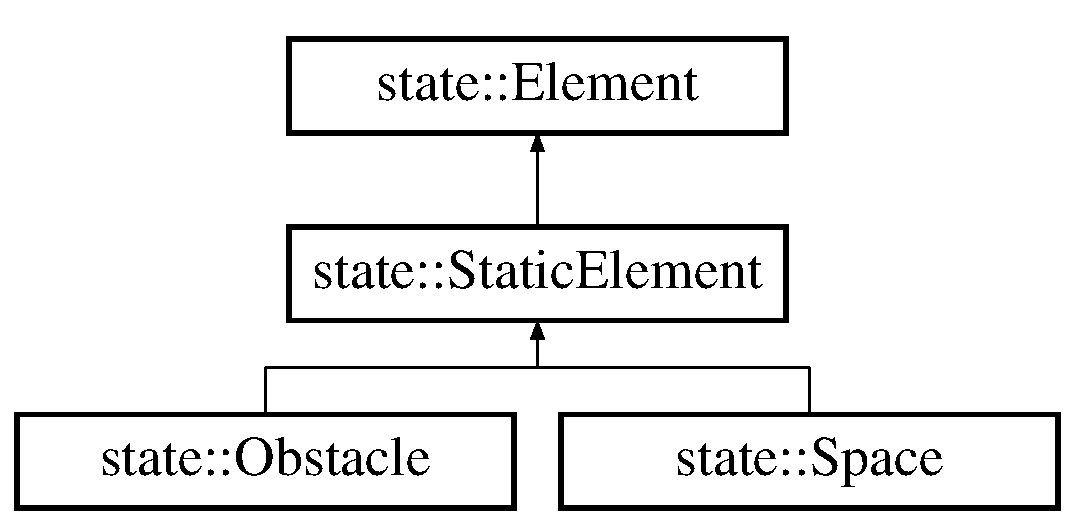
\includegraphics[height=3.000000cm]{classstate_1_1_static_element}
\end{center}
\end{figure}
\subsection*{Public Member Functions}
\begin{DoxyCompactItemize}
\item 
\mbox{\Hypertarget{classstate_1_1_static_element_a2b96c76d0a9b0b9ef5b492cfc607cf57}\label{classstate_1_1_static_element_a2b96c76d0a9b0b9ef5b492cfc607cf57}} 
bool \hyperlink{classstate_1_1_static_element_a2b96c76d0a9b0b9ef5b492cfc607cf57}{is\+Static} () const
\begin{DoxyCompactList}\small\item\em class \hyperlink{classstate_1_1_static_element}{Static\+Element} -\/ \end{DoxyCompactList}\item 
\mbox{\Hypertarget{classstate_1_1_static_element_a26612ed9b6442a92d4f8f4a6696db8ec}\label{classstate_1_1_static_element_a26612ed9b6442a92d4f8f4a6696db8ec}} 
virtual bool {\bfseries is\+Space} () const =0
\end{DoxyCompactItemize}
\subsection*{Additional Inherited Members}


\subsection{Detailed Description}
class \hyperlink{classstate_1_1_static_element}{Static\+Element} -\/ 

The documentation for this class was generated from the following files\+:\begin{DoxyCompactItemize}
\item 
C\+:/\+Users/corentin/\+Desktop/projet tank/src modif/\+Tank\+State/include/Static\+Element.\+h\item 
C\+:/\+Users/corentin/\+Desktop/projet tank/src modif/\+Tank\+State/src/Static\+Element.\+cpp\end{DoxyCompactItemize}

\hypertarget{classstate_1_1_tank}{}\section{state\+:\+:Tank Class Reference}
\label{classstate_1_1_tank}\index{state\+::\+Tank@{state\+::\+Tank}}


class \hyperlink{classstate_1_1_tank}{Tank} -\/  




{\ttfamily \#include $<$Tank.\+h$>$}

Inheritance diagram for state\+:\+:Tank\+:\begin{figure}[H]
\begin{center}
\leavevmode
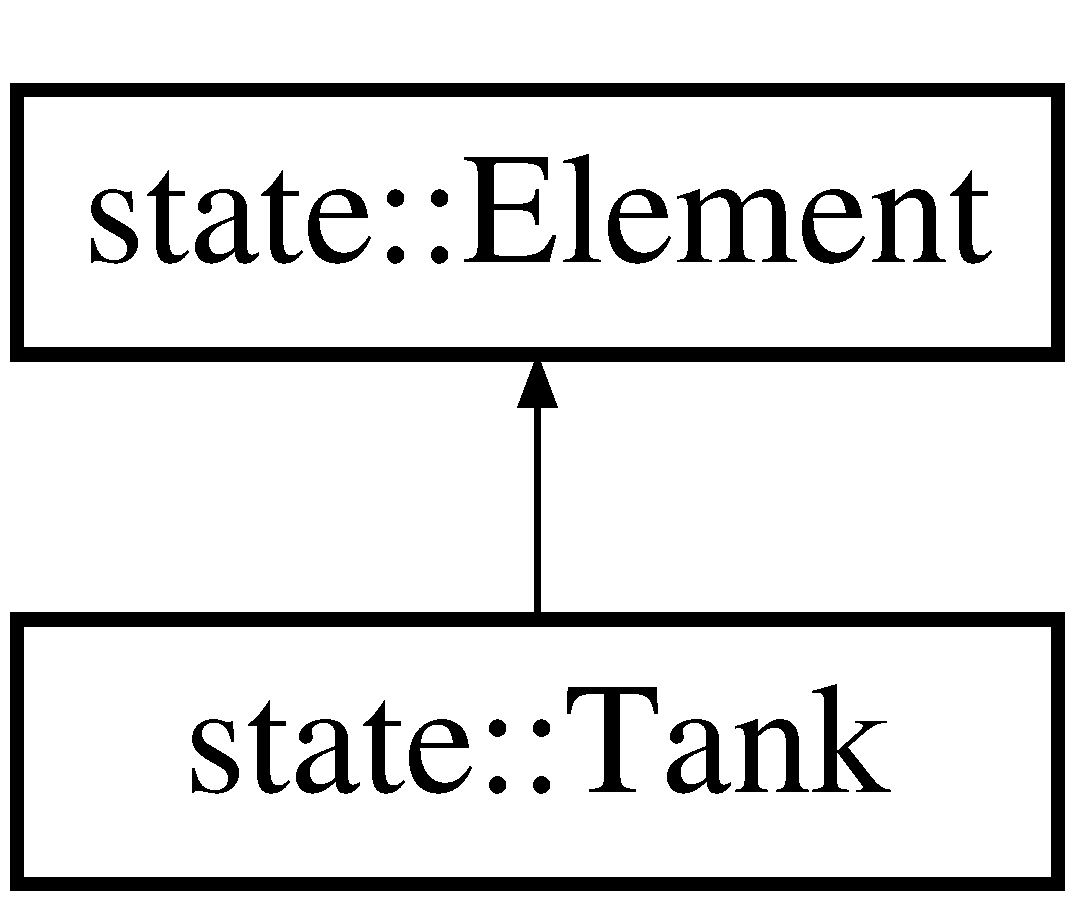
\includegraphics[height=2.000000cm]{classstate_1_1_tank}
\end{center}
\end{figure}
\subsection*{Public Member Functions}
\begin{DoxyCompactItemize}
\item 
\mbox{\Hypertarget{classstate_1_1_tank_aa06104e09cb1fd7c92159babf64a9b54}\label{classstate_1_1_tank_aa06104e09cb1fd7c92159babf64a9b54}} 
{\bfseries Tank} (Tank\+Type\+Id tanktypeid, Orientation orientation, int x, int y)
\item 
\mbox{\Hypertarget{classstate_1_1_tank_a3a0342c57ef771c0bb3f04cede384891}\label{classstate_1_1_tank_a3a0342c57ef771c0bb3f04cede384891}} 
bool {\bfseries is\+Static} () const
\item 
\mbox{\Hypertarget{classstate_1_1_tank_ab1c8d302d263e6461c633477dc92473a}\label{classstate_1_1_tank_ab1c8d302d263e6461c633477dc92473a}} 
Type\+Id {\bfseries get\+Type\+Id} () const
\item 
\mbox{\Hypertarget{classstate_1_1_tank_a11a64c116f8bed48f8d73f5712cd073e}\label{classstate_1_1_tank_a11a64c116f8bed48f8d73f5712cd073e}} 
void {\bfseries set\+Pv} (int pv)
\item 
\mbox{\Hypertarget{classstate_1_1_tank_a4c567fbc4dfe80c8f342d5fc7d74bcf3}\label{classstate_1_1_tank_a4c567fbc4dfe80c8f342d5fc7d74bcf3}} 
int {\bfseries get\+Pv} () const
\item 
\mbox{\Hypertarget{classstate_1_1_tank_aca6c9a90d94a81d0d95dabeb1d378297}\label{classstate_1_1_tank_aca6c9a90d94a81d0d95dabeb1d378297}} 
Orientation {\bfseries get\+Orientation} () const
\item 
\mbox{\Hypertarget{classstate_1_1_tank_ae74c06cfa4e5fdd8834670d3019f770b}\label{classstate_1_1_tank_ae74c06cfa4e5fdd8834670d3019f770b}} 
void {\bfseries set\+Orientation} (Orientation o)
\item 
\mbox{\Hypertarget{classstate_1_1_tank_a091c2f4a6d33caee15602706d2ab0ffa}\label{classstate_1_1_tank_a091c2f4a6d33caee15602706d2ab0ffa}} 
void {\bfseries set\+Tank\+Type\+Id} (Tank\+Type\+Id id)
\item 
\mbox{\Hypertarget{classstate_1_1_tank_a5abc3898a0b6c4ab279111222afd4555}\label{classstate_1_1_tank_a5abc3898a0b6c4ab279111222afd4555}} 
Tank\+Type\+Id {\bfseries get\+Tank\+Type\+Id} () const
\item 
\mbox{\Hypertarget{classstate_1_1_tank_a088768d906ca877fda341ce9eab04882}\label{classstate_1_1_tank_a088768d906ca877fda341ce9eab04882}} 
\hyperlink{classstate_1_1_element}{Element} $\ast$ {\bfseries clone} () const
\end{DoxyCompactItemize}
\subsection*{Protected Attributes}
\begin{DoxyCompactItemize}
\item 
\mbox{\Hypertarget{classstate_1_1_tank_acfb1b29669978895d80ebedcc661ba52}\label{classstate_1_1_tank_acfb1b29669978895d80ebedcc661ba52}} 
int {\bfseries pv}
\end{DoxyCompactItemize}


\subsection{Detailed Description}
class \hyperlink{classstate_1_1_tank}{Tank} -\/ 

The documentation for this class was generated from the following files\+:\begin{DoxyCompactItemize}
\item 
C\+:/\+Users/corentin/\+Desktop/projet tank/src modif/\+Tank\+State/include/Tank.\+h\item 
C\+:/\+Users/corentin/\+Desktop/projet tank/src modif/\+Tank\+State/src/Tank.\+cpp\end{DoxyCompactItemize}

\chapter{File Documentation}
\hypertarget{_space_8cpp}{}\section{C\+:/\+Users/corentin/\+Desktop/projet tank/src modif/\+Tank\+State/src/\+Space.cpp File Reference}
\label{_space_8cpp}\index{C\+:/\+Users/corentin/\+Desktop/projet tank/src modif/\+Tank\+State/src/\+Space.\+cpp@{C\+:/\+Users/corentin/\+Desktop/projet tank/src modif/\+Tank\+State/src/\+Space.\+cpp}}


Element Space.  


{\ttfamily \#include \char`\"{}Space.\+h\char`\"{}}\newline
\subsection*{Namespaces}
\begin{DoxyCompactItemize}
\item 
 \hyperlink{namespacestate}{state}
\begin{DoxyCompactList}\small\item\em Espace de nommage regroupant les données représentant l\textquotesingle{}état du jeu. \end{DoxyCompactList}\end{DoxyCompactItemize}


\subsection{Detailed Description}
Element Space. 

\begin{DoxyAuthor}{Author}
Corentin.\+M 
\end{DoxyAuthor}
\begin{DoxyVersion}{Version}
0.\+1 
\end{DoxyVersion}
\begin{DoxyDate}{Date}
17 février 2017
\end{DoxyDate}
Element symbolisant les cases traversables dans le jeu. 
%--- End generated contents ---

% Index
\backmatter
\newpage
\phantomsection
\clearemptydoublepage
\addcontentsline{toc}{chapter}{Index}
\printindex

\end{document}
